\documentclass[aspectratio=1610]{beamer}
\usepackage{graphicx}

\graphicspath{{./openTOPAS/}}
\DeclareRobustCommand\SUTname{TOPAS-nBio (TOPAS v3.5)}
\DeclareRobustCommand\benchmarkname{TOPAS-nBio (TOPAS v3.4)}


\title{\SUTname}
\subtitle{Regression testing (cf.\ \benchmarkname)}
\author{Jos\'e Ramos-M\'endez and Thongchai A.M. Masilela}
\institute{University of California San Francisco}
\date{\today}



\begin{document}

\frame{\titlepage}

%\begin{frame}
 % \frametitle{Table of contents}
  %\tableofcontents
%\end{frame}

\begin{frame}[allowframebreaks]{Table of Contents}
  \tableofcontents[sections={1-11}]
    \framebreak
  \tableofcontents[sections={12-}]
\end{frame}

\section{DBSCAN - TsEmDNAPhysics}

\begin{frame}{\secname}
 \begin{columns}
  \begin{column}{0.4\linewidth}
   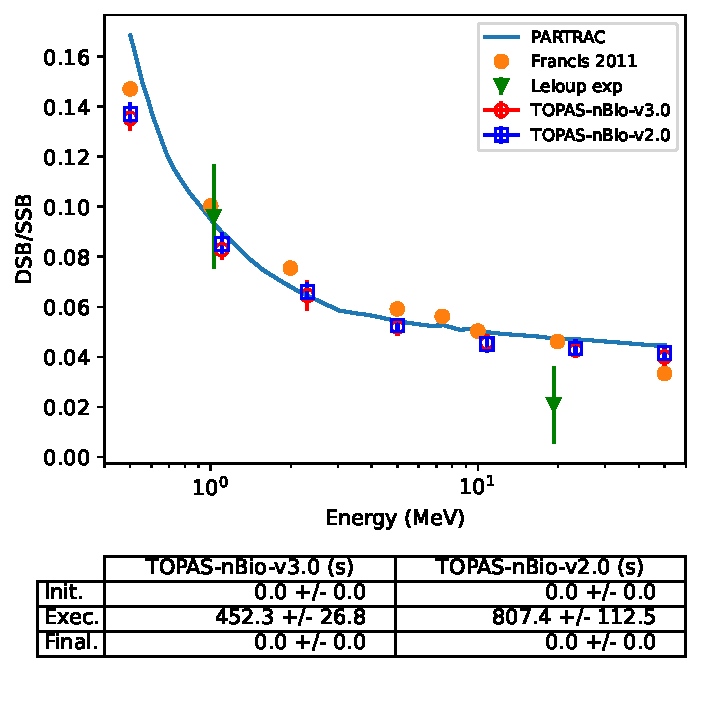
\includegraphics[width=1.1\textwidth]{./DBSCAN/DBSCAN2_TsEmDNAPhysics}
  \end{column}
  \begin{column}{0.6\linewidth} 
   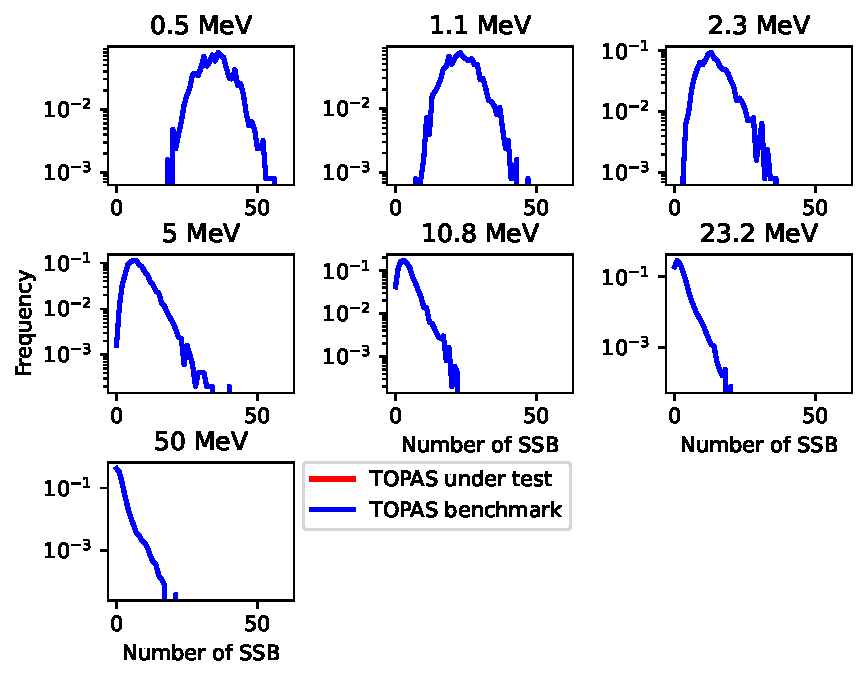
\includegraphics[width=\textwidth]{./DBSCAN/DBSCAN1_TsEmDNAPhysics}
  \end{column}
 \end{columns}
\begin{itemize}
\item \tiny{Francis Z, Villagrasa C, Clairand I. Simulation of DNA damage clustering after proton irradiation using an adapted DBSCAN algorithm. \textit{Comput Methods Programs Biomed}. 2011; 101(3):265-270. doi:10.1016/j.cmpb.2010.12.012}
\end{itemize}
\end{frame}

\section{DBSCAN - g4em-dna$\_$opt2}

\begin{frame}{\secname}
 \begin{columns}
  \begin{column}{0.4\linewidth}
   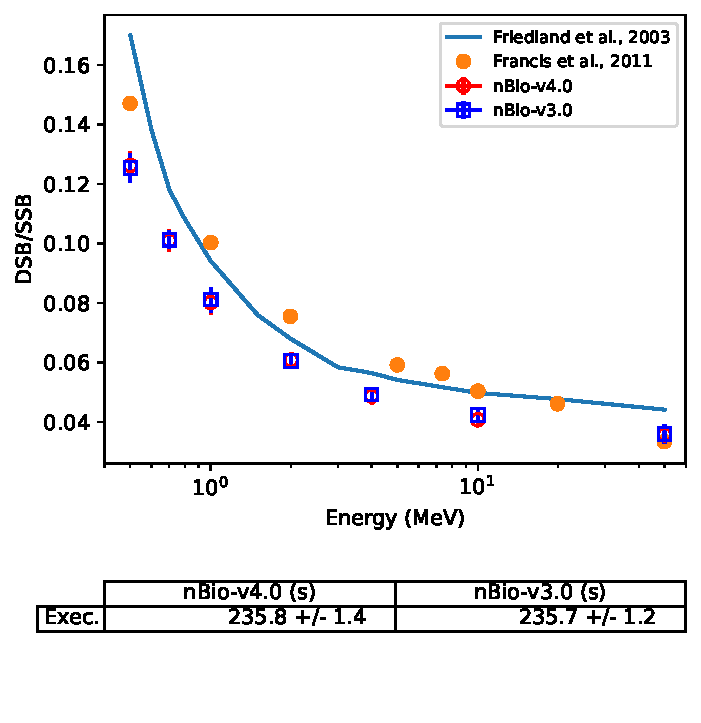
\includegraphics[width=1.1\textwidth]{./DBSCAN/DBSCAN2_g4em-dna_opt2}
  \end{column}
  \begin{column}{0.6\linewidth} 
   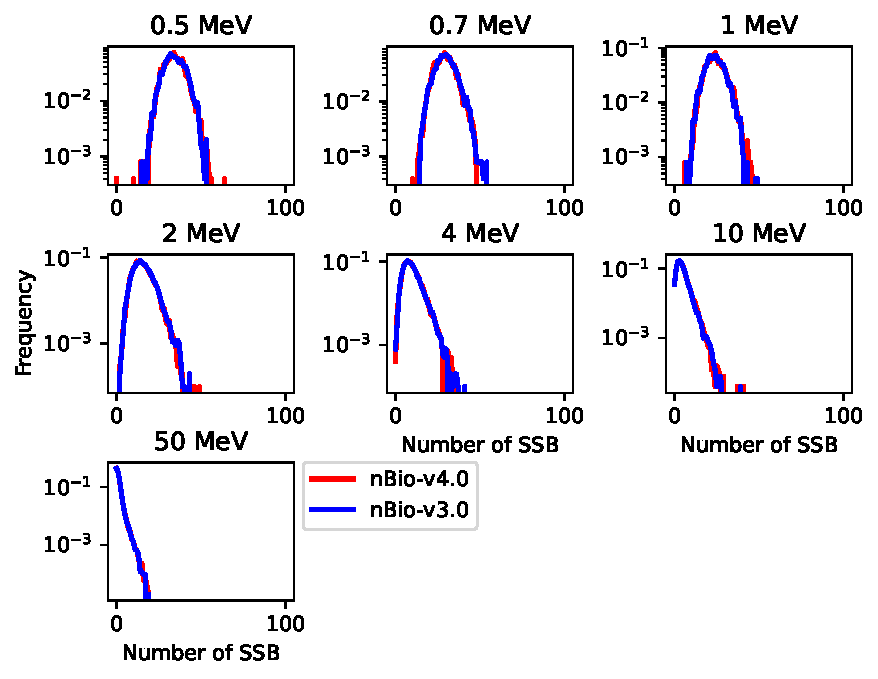
\includegraphics[width=\textwidth]{./DBSCAN/DBSCAN1_g4em-dna_opt2}
  \end{column}
 \end{columns}
\begin{itemize}
\item \tiny{Francis Z, Villagrasa C, Clairand I. Simulation of DNA damage clustering after proton irradiation using an adapted DBSCAN algorithm. \textit{Comput Methods Programs Biomed}. 2011; 101(3):265-270. doi:10.1016/j.cmpb.2010.12.012}
\end{itemize}
\end{frame}

\section{DBSCAN - g4em-dna$\_$opt4}

\begin{frame}{\secname}
 \begin{columns}
  \begin{column}{0.4\linewidth}
   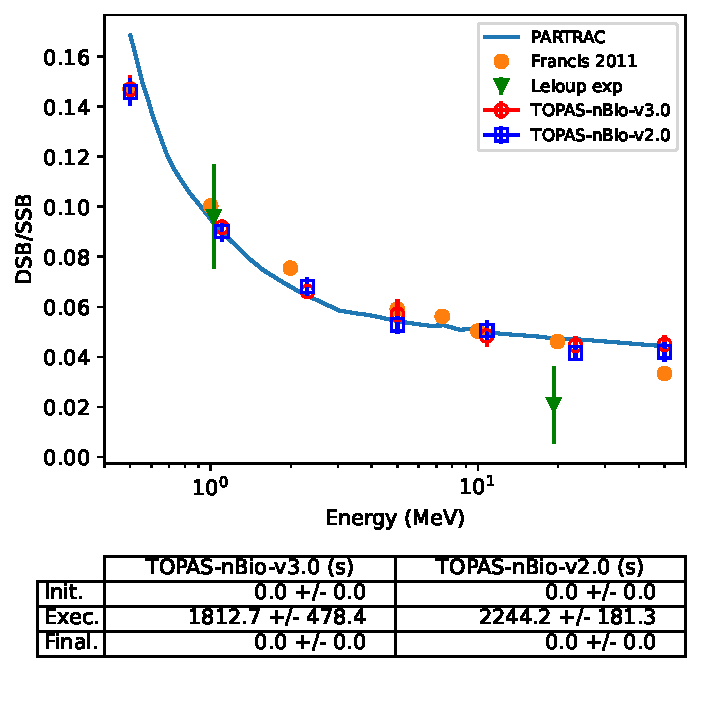
\includegraphics[width=1.1\textwidth]{./DBSCAN/DBSCAN2_g4em-dna_opt4}
  \end{column}
  \begin{column}{0.6\linewidth} 
   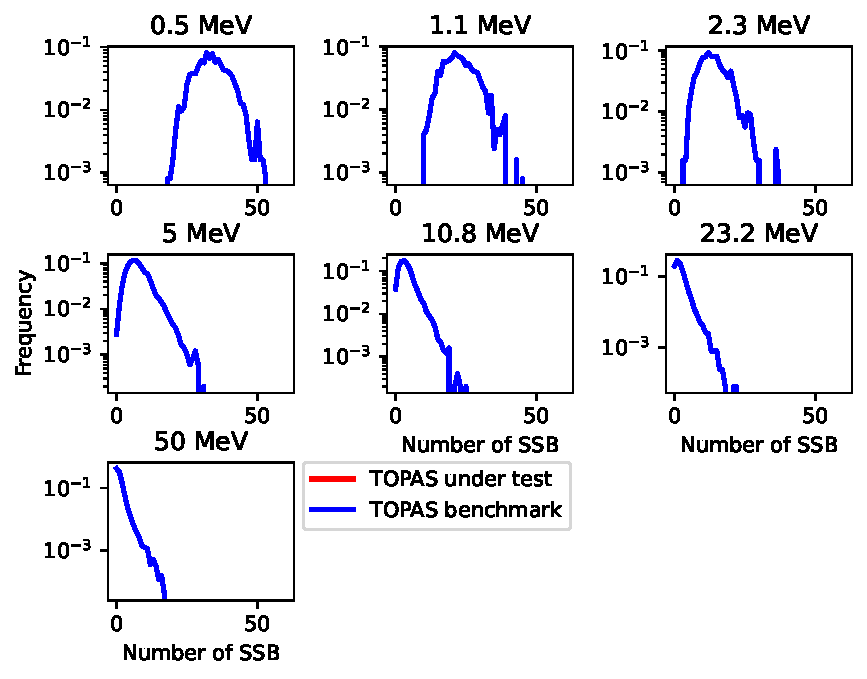
\includegraphics[width=\textwidth]{./DBSCAN/DBSCAN1_g4em-dna_opt4}
  \end{column}
 \end{columns}
\begin{itemize}
\item \tiny{Francis Z, Villagrasa C, Clairand I. Simulation of DNA damage clustering after proton irradiation using an adapted DBSCAN algorithm. \textit{Comput Methods Programs Biomed}. 2011; 101(3):265-270. doi:10.1016/j.cmpb.2010.12.012}
\end{itemize}
\end{frame}

\section{DBSCAN - g4em-dna\_opt6}

\begin{frame}{\secname}
 \begin{columns}
  \begin{column}{0.4\linewidth}
   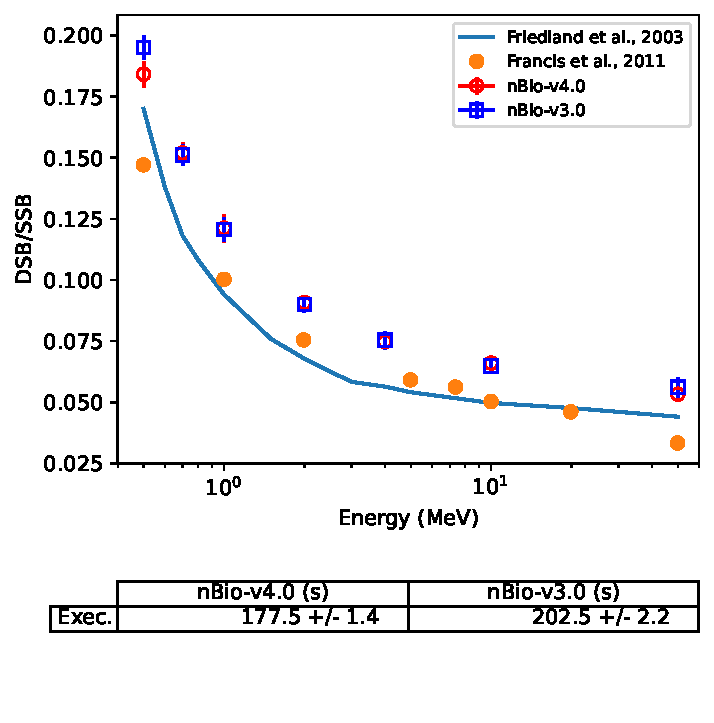
\includegraphics[width=1.1\textwidth]{./DBSCAN/DBSCAN2_g4em-dna_opt6}
  \end{column}
  \begin{column}{0.6\linewidth} 
   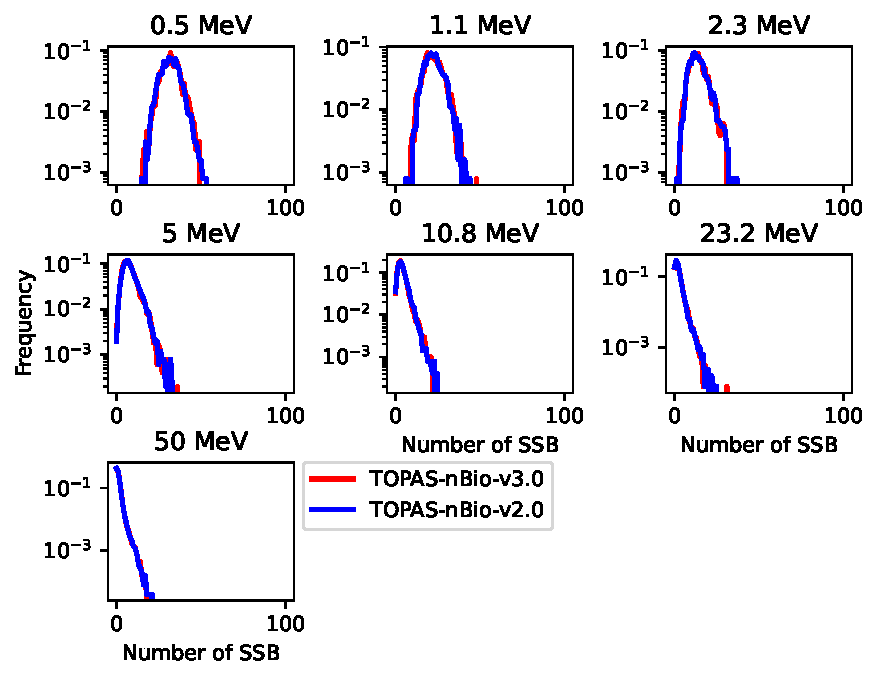
\includegraphics[width=\textwidth]{./DBSCAN/DBSCAN1_g4em-dna_opt6}
  \end{column}
 \end{columns}
\begin{itemize}
\item \tiny{Francis Z, Villagrasa C, Clairand I. Simulation of DNA damage clustering after proton irradiation using an adapted DBSCAN algorithm. \textit{Comput Methods Programs Biomed}. 2011; 101(3):265-270. doi:10.1016/j.cmpb.2010.12.012}
\end{itemize}
\end{frame}

\section{LET I}

\begin{frame}{\secname}
  \begin{columns}
    \begin{column}{0.4\linewidth}
     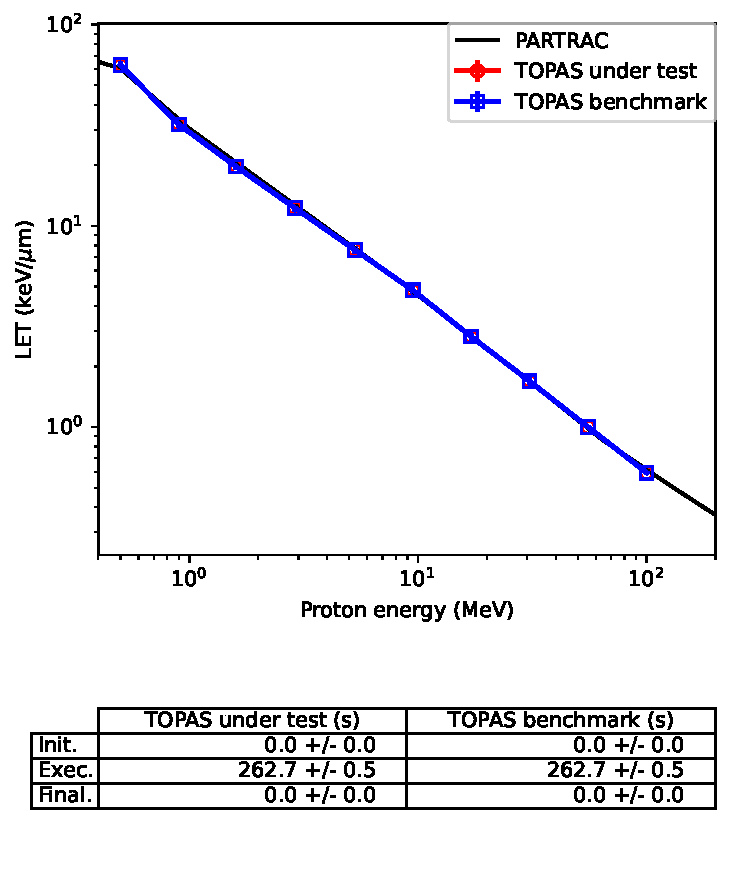
\includegraphics[width=\textwidth]{./LET/LET_TsEmDNAPhysics}
    \end{column}
    \begin{column}{0.4\linewidth} 
     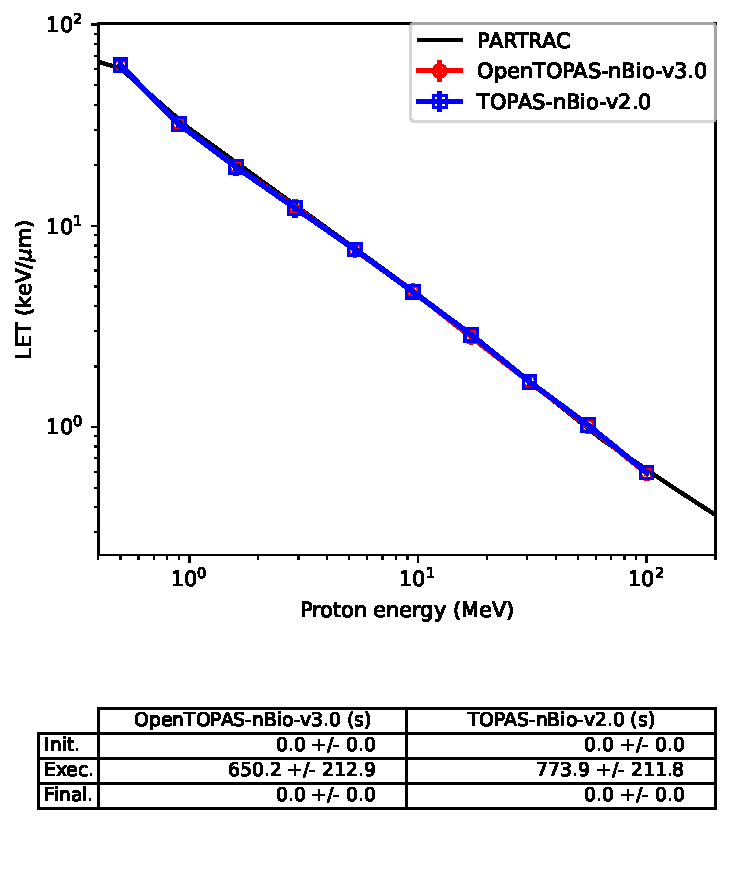
\includegraphics[width=\textwidth]{./LET/LET_g4em-dna_opt2}
    \end{column}
   \end{columns}
\begin{itemize}
\item \tiny{LET as a function of proton energy for TsEmDNAPhysics (left) and g4em-dna\_opt2 (right).}
\end{itemize}
\end{frame}

\section{LET II}

\begin{frame}{\secname}
  \begin{columns}
    \begin{column}{0.4\linewidth}
     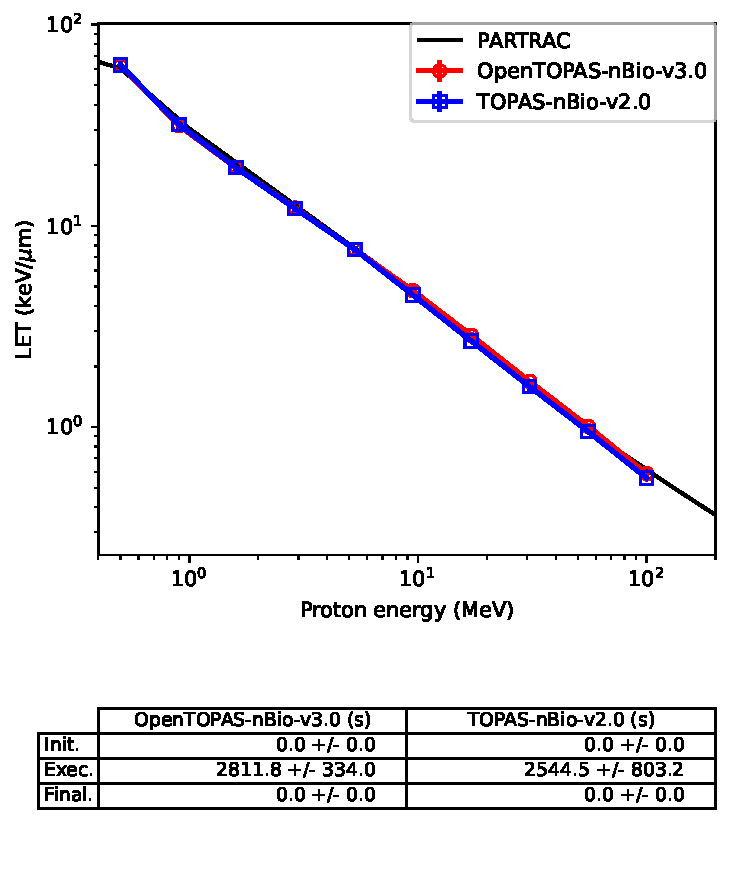
\includegraphics[width=\textwidth]{./LET/LET_g4em-dna_opt4}
    \end{column}
    \begin{column}{0.4\linewidth} 
     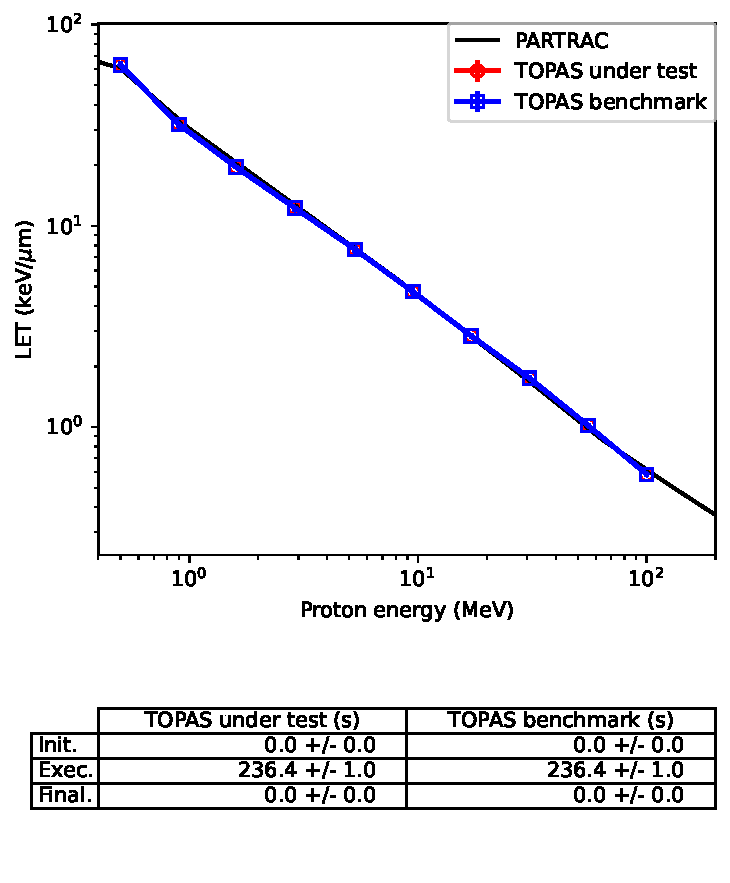
\includegraphics[width=\textwidth]{./LET/LET_g4em-dna_opt6}
    \end{column}
   \end{columns}
\begin{itemize}
\item \tiny{LET as a function of proton energy for g4em-dna\_opt4 (left) and g4em-dna\_opt6 (right).}
\end{itemize}
\end{frame}

\section{Fricke: IRT}

\begin{frame}{\secname}
 \centering
  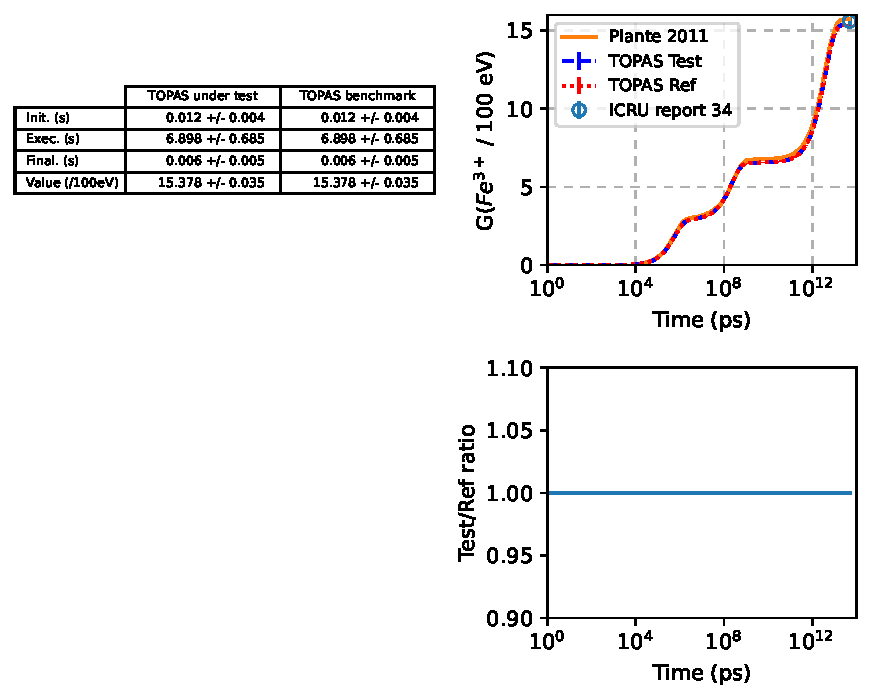
\includegraphics[width=0.75\textwidth]{./frickeIRT/Gvalue}
\end{frame}

\section{G-value: step-by-step}

\begin{frame}{\secname}
 \centering
   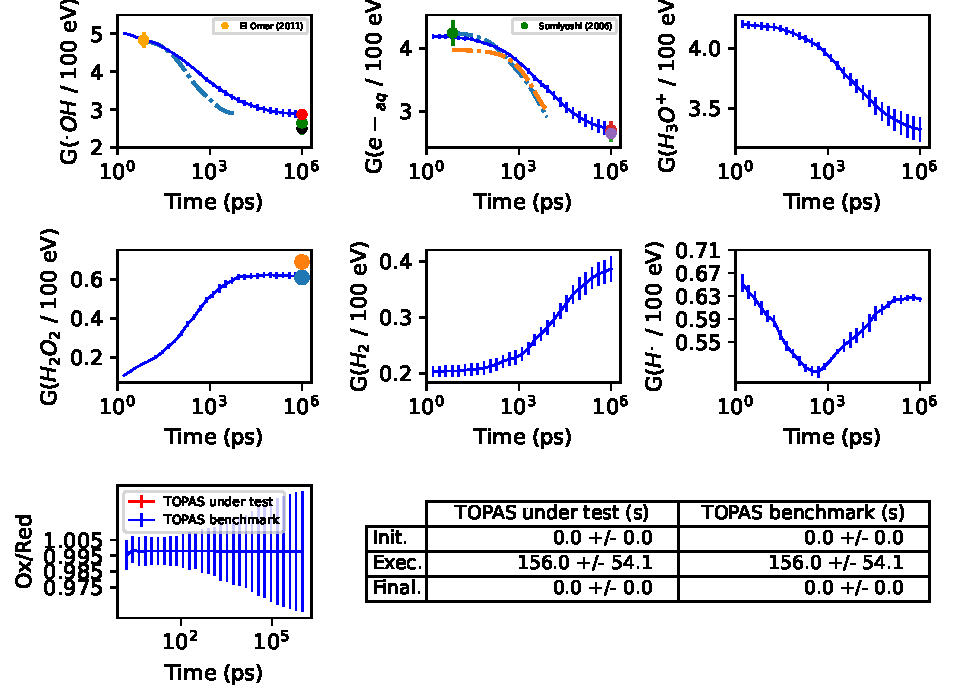
\includegraphics[width=0.75\textwidth]{./gvalueSBS/Gvalue}
\end{frame}

\section{G-value vs. LET: step-by-step}

\begin{frame}{\secname}
 \centering
   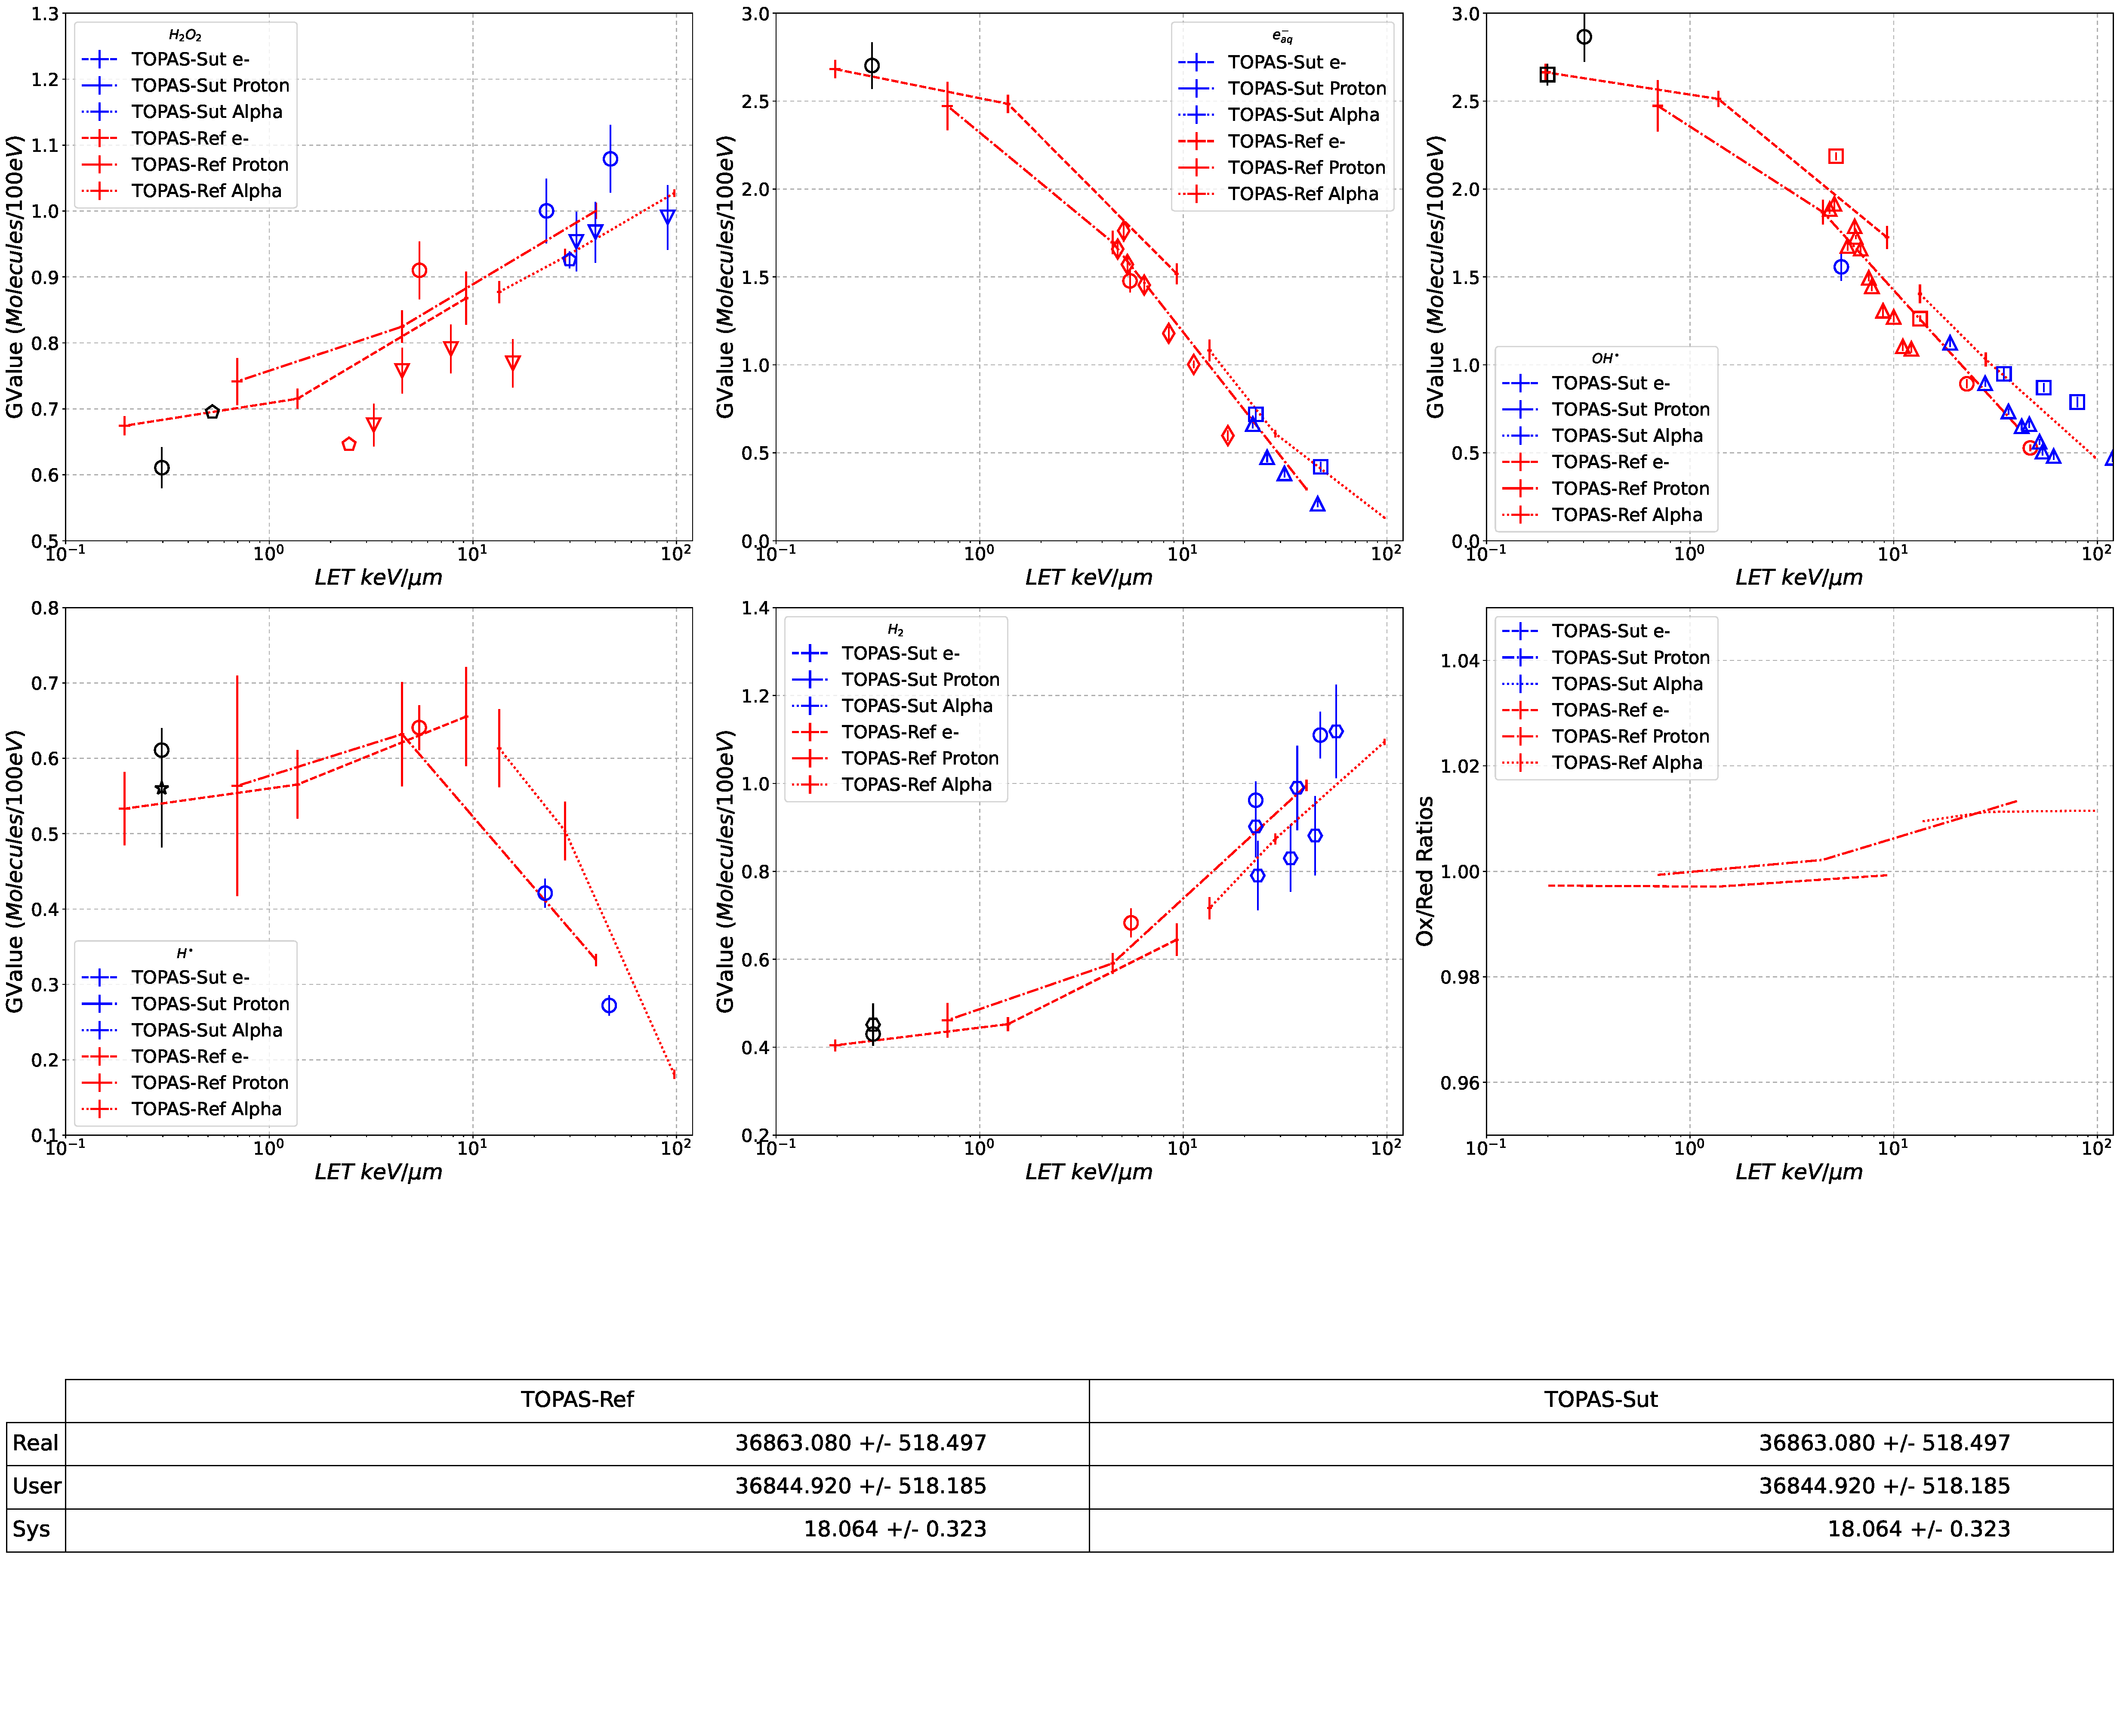
\includegraphics[width=0.75\textwidth]{./gvalue_LET_SBS/Gvalue_LET-SBS}
\end{frame}

\section{G-value: IRT}

\begin{frame}{\secname}
 \centering
  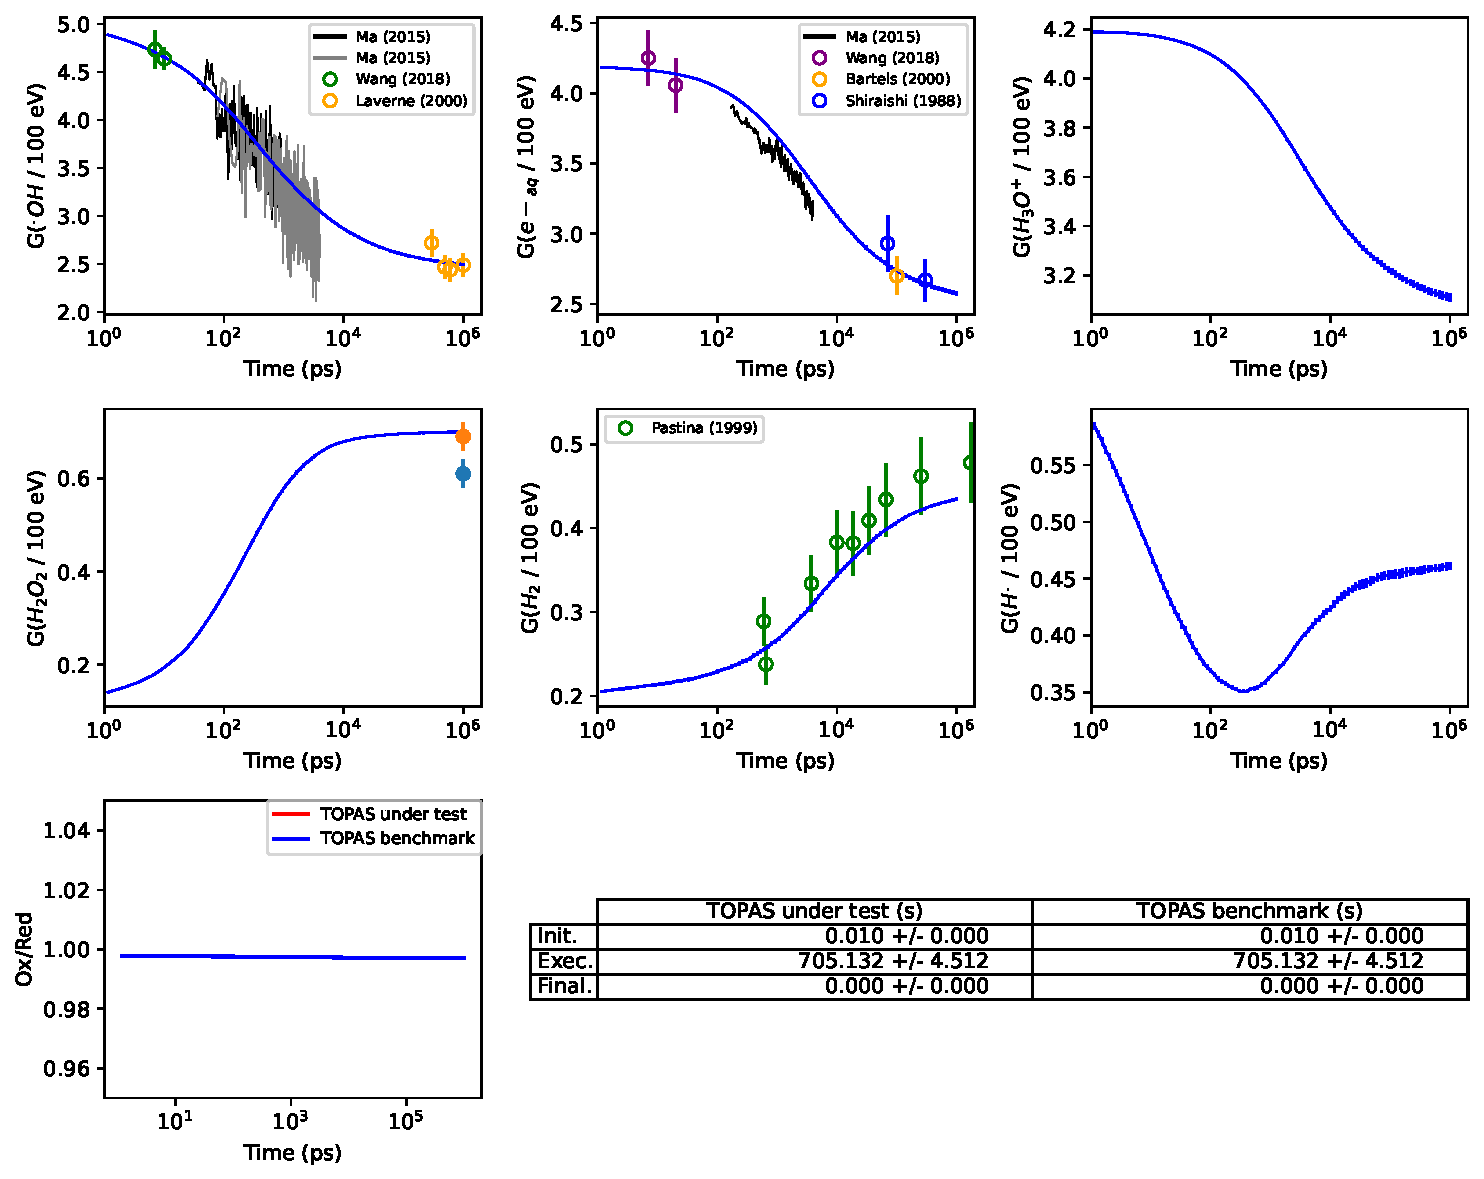
\includegraphics[width=0.75\textwidth]{./gvalueIRT/GvalueIRT}
\end{frame}

\section{G-value vs. LET: IRT}

\begin{frame}{\secname}
 \centering
  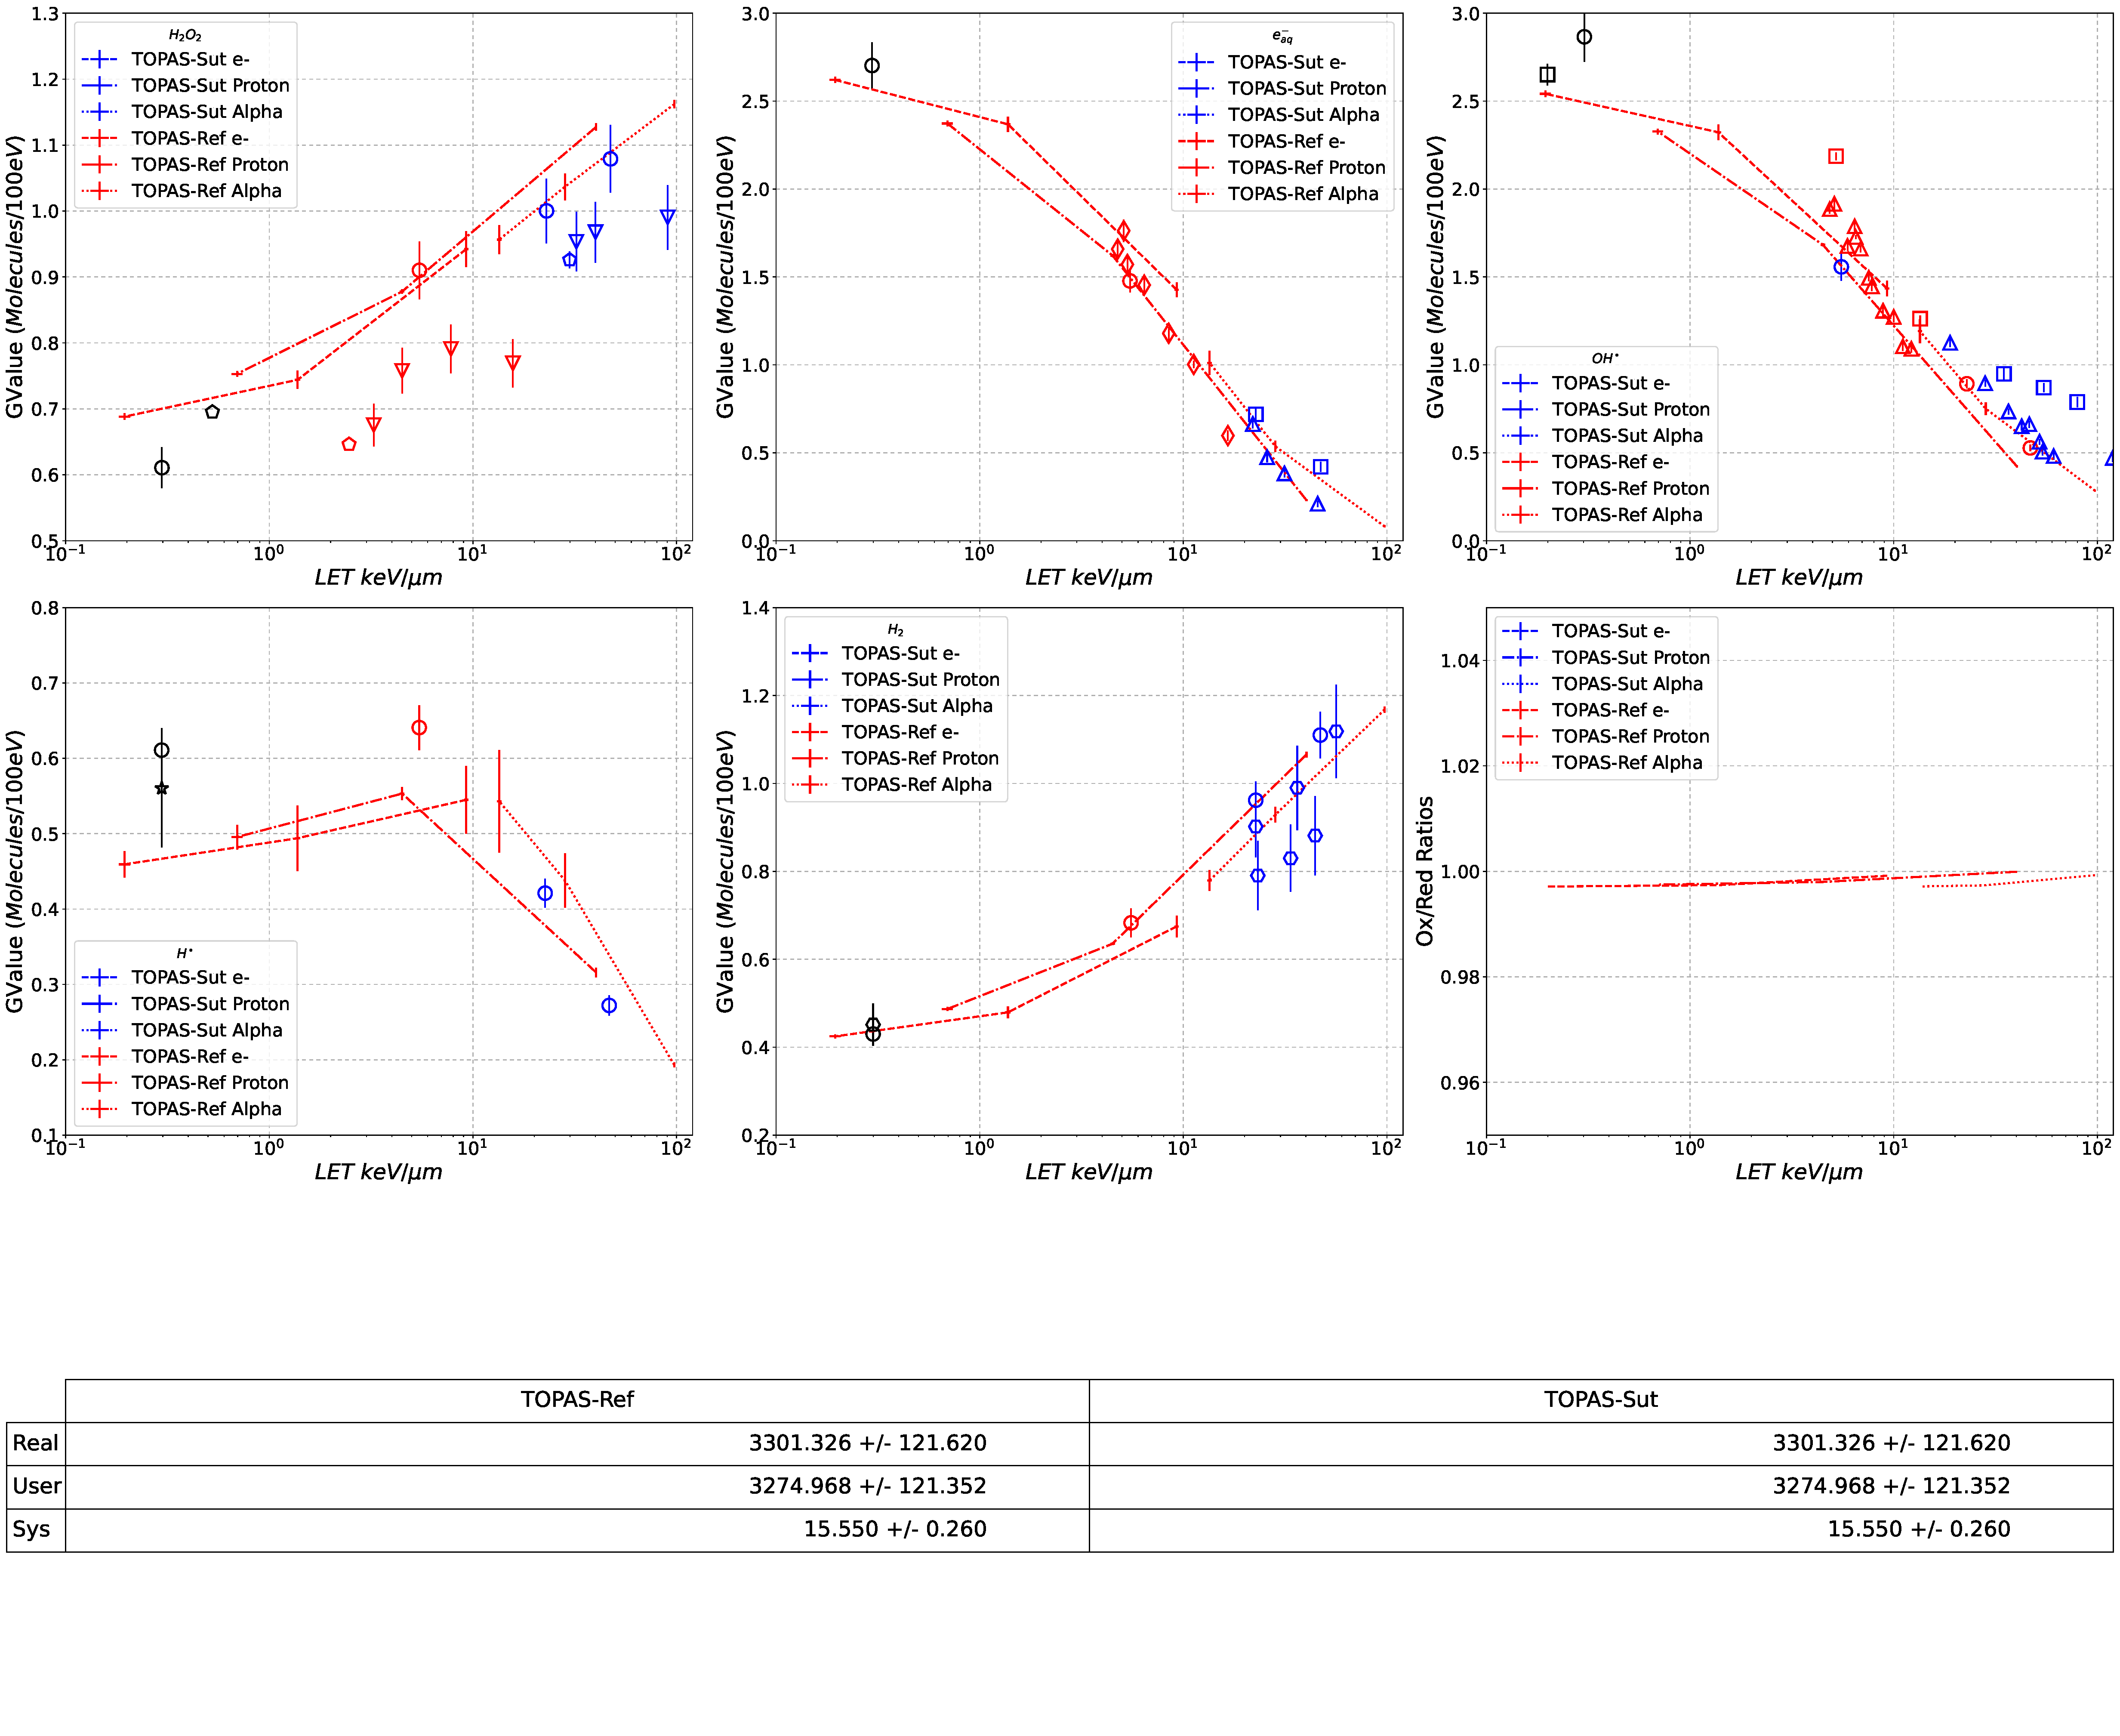
\includegraphics[width=0.75\textwidth]{./gvalue_LET_IRT/Gvalue_LET-IRT}
\end{frame}

\section{G-value of H$_2$O$_2$: IRT}

\begin{frame}{\secname}
 \centering
  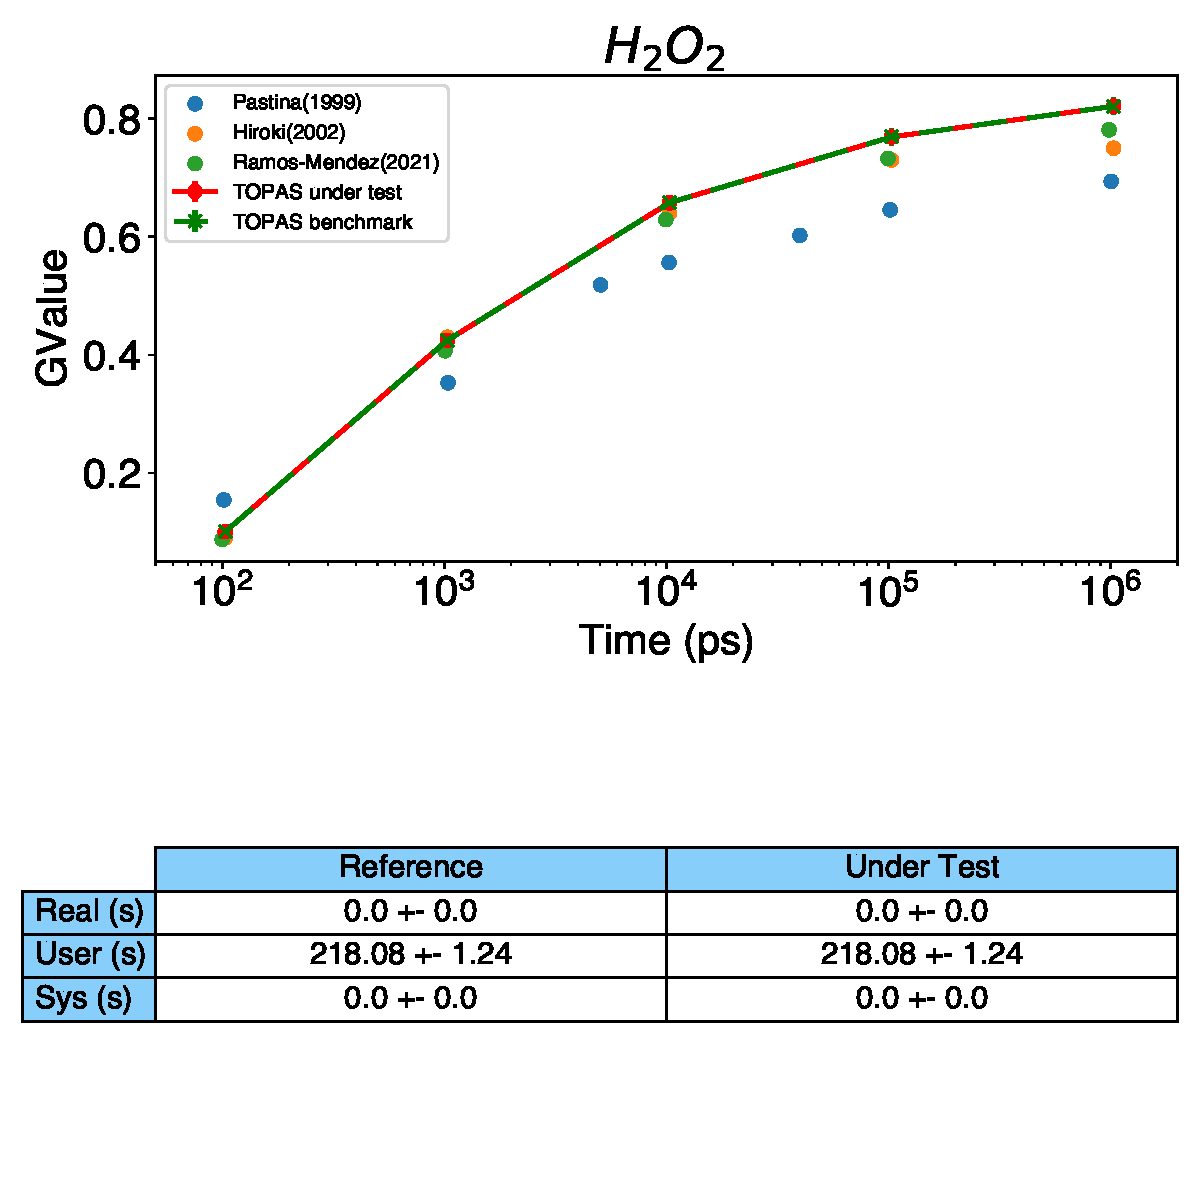
\includegraphics[width=0.6\textwidth]{./gvalueIRT_H2O2/TimeEvolution}
\end{frame}

\section{G-value and Temperature I: IRT}

\begin{frame}{\secname}
 \centering
  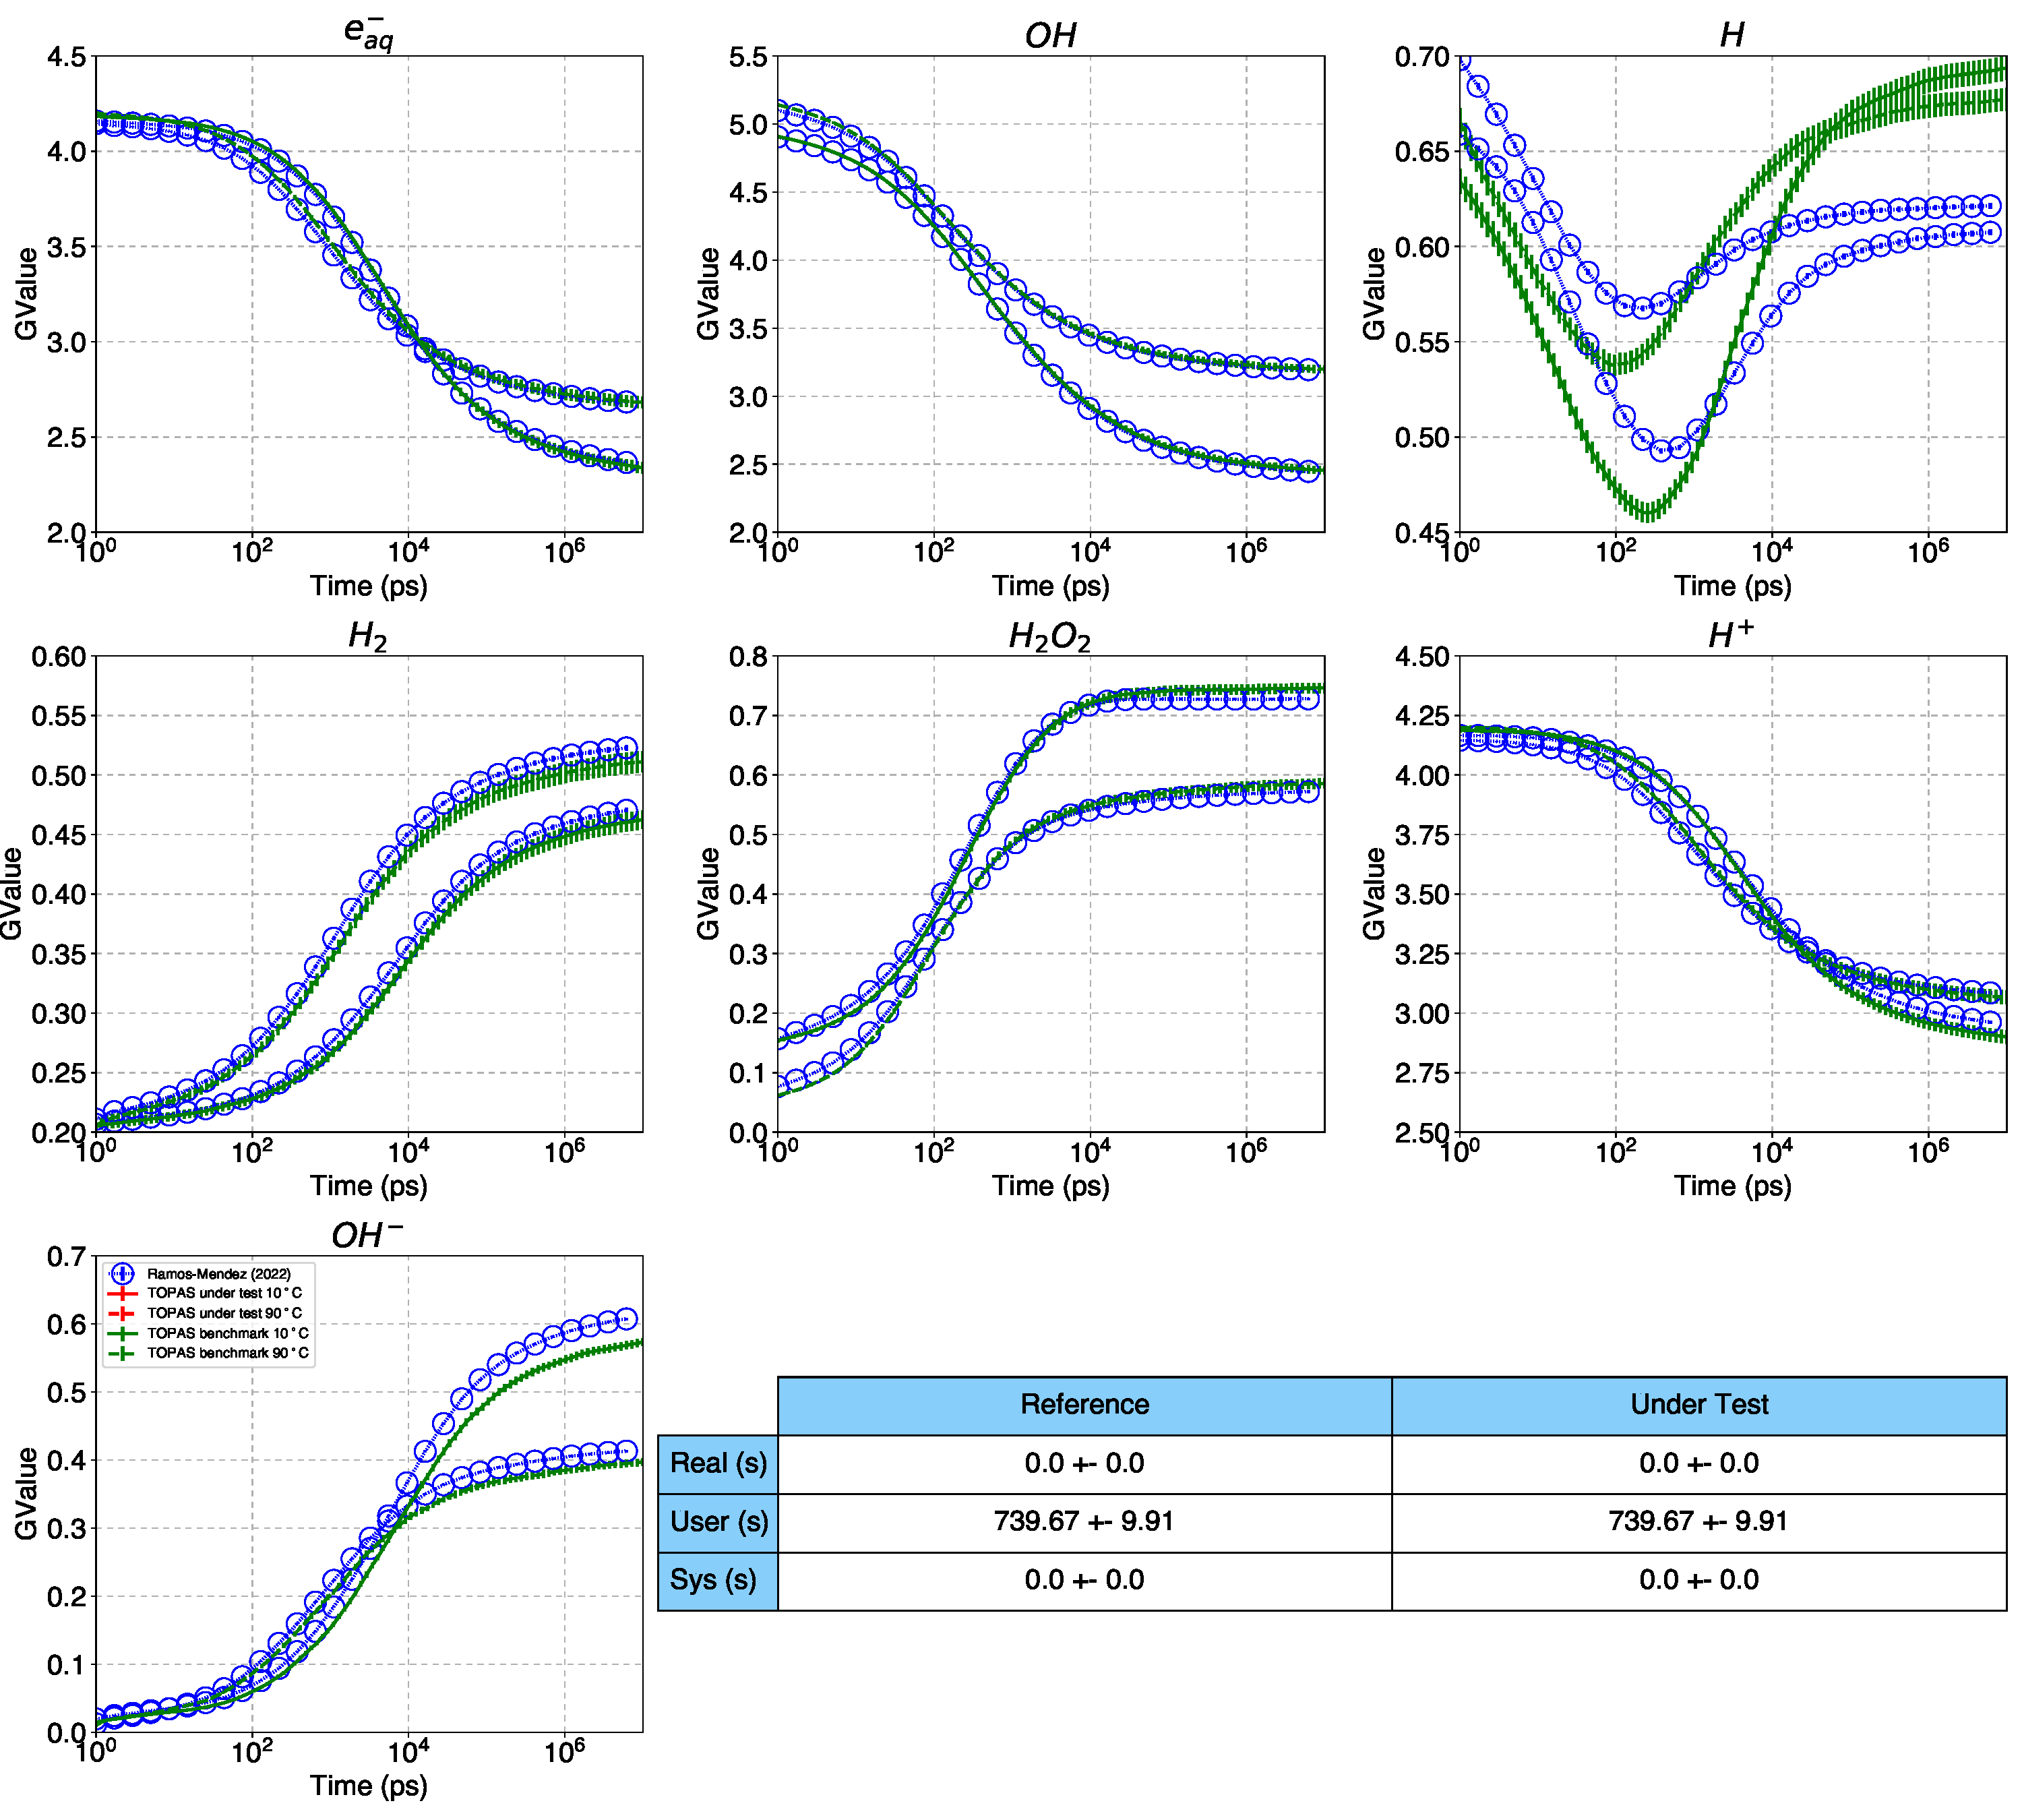
\includegraphics[width=0.7\textwidth]{./gvalueIRT_temp/TimeEvolution}
\end{frame}

\section{G-value and Temperature II: IRT}

\begin{frame}{\secname}
 \centering
  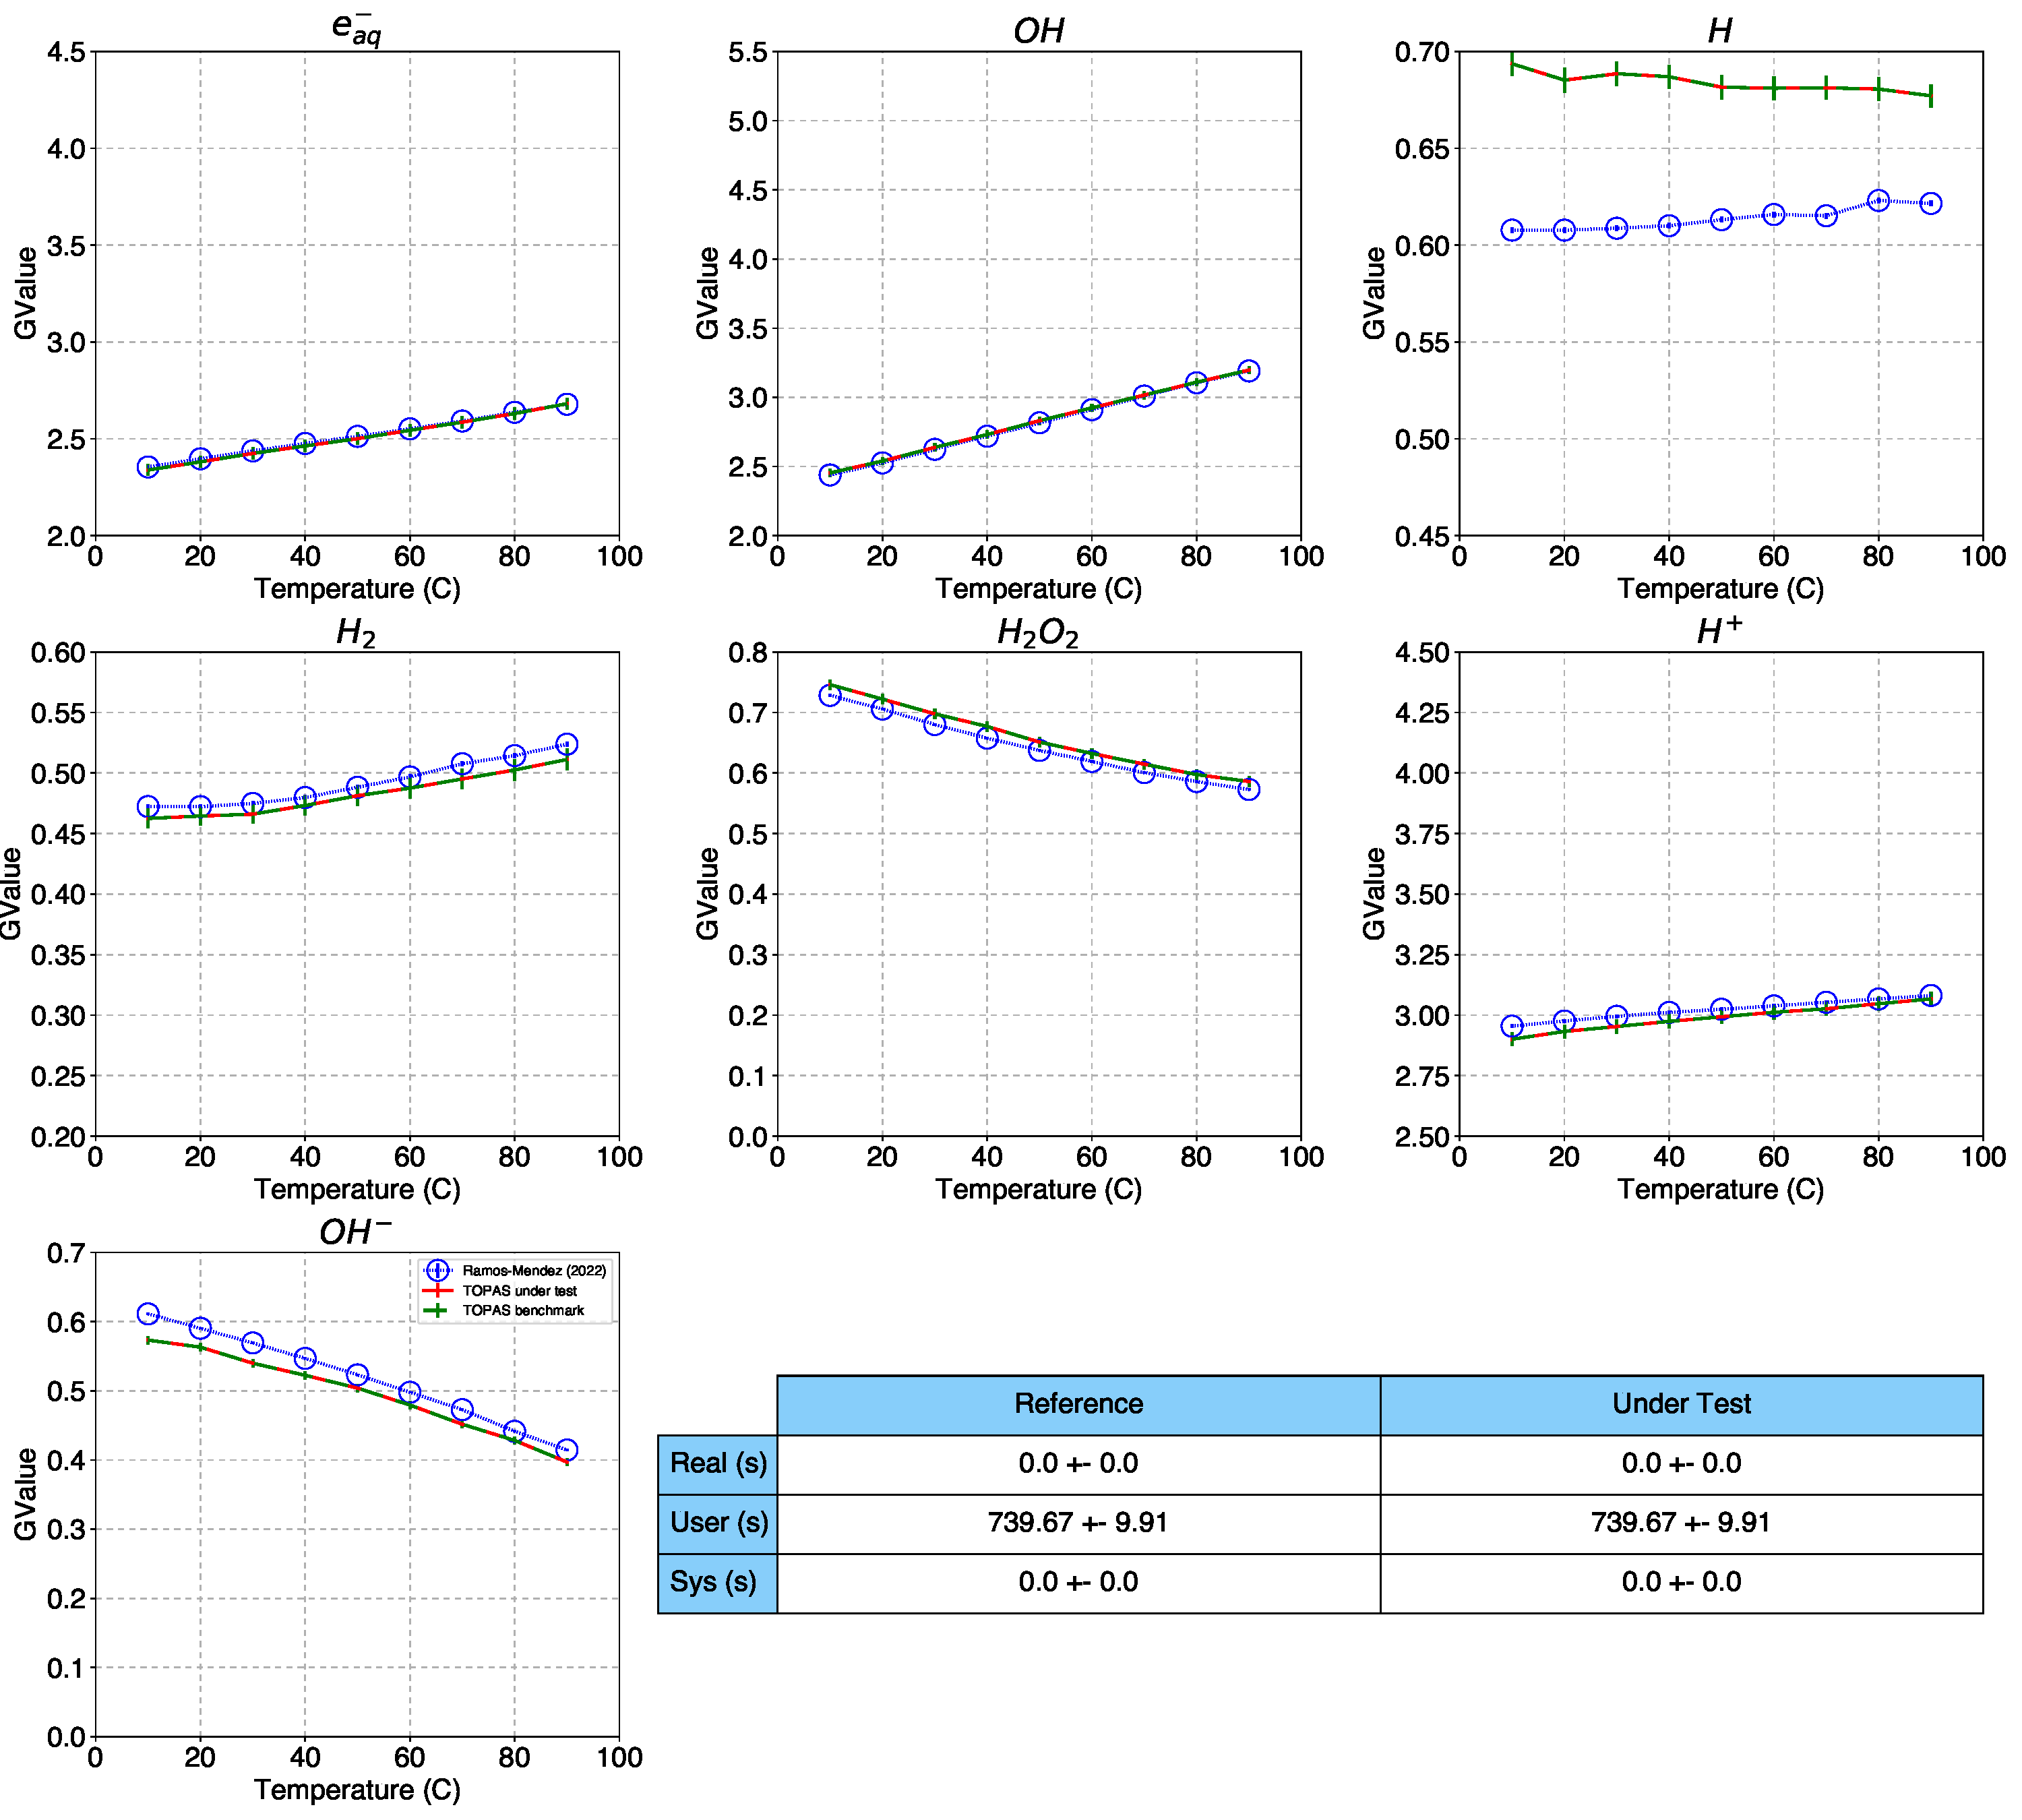
\includegraphics[width=0.7\textwidth]{./gvalueIRT_temp/TemperatureEvolution}
\end{frame}

\section{Nanodosimetry I: TsEmDNAPhysics and g4em-dna\_opt2}

\begin{frame}{\secname}
  \begin{columns}
    \begin{column}{0.4\linewidth}
     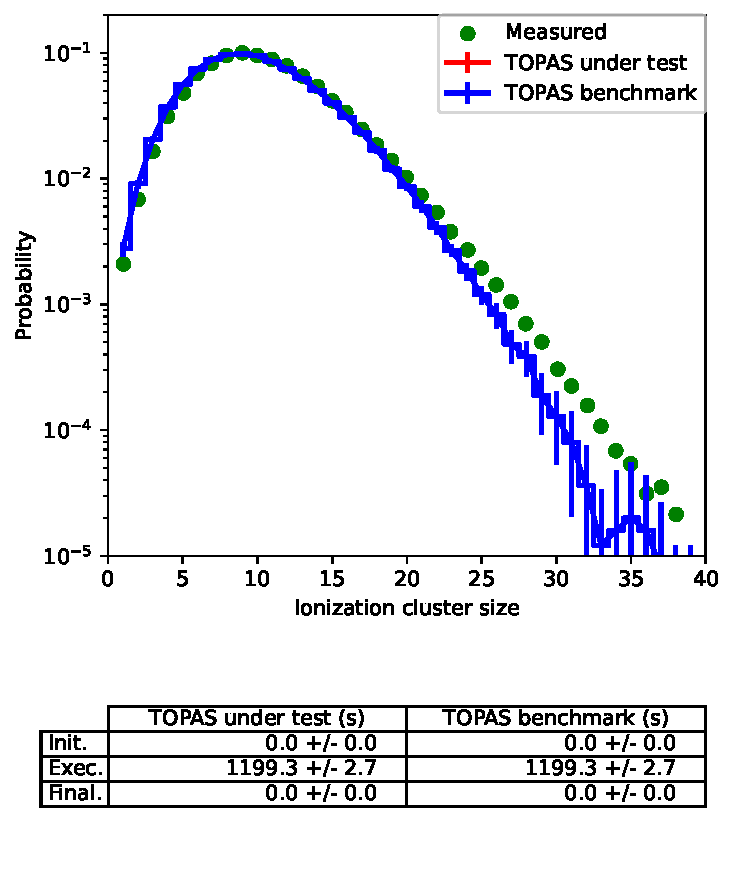
\includegraphics[width=\textwidth]{./nano1/IDDistribution_TsEmDNAPhysics}
    \end{column}
    \begin{column}{0.4\linewidth} 
     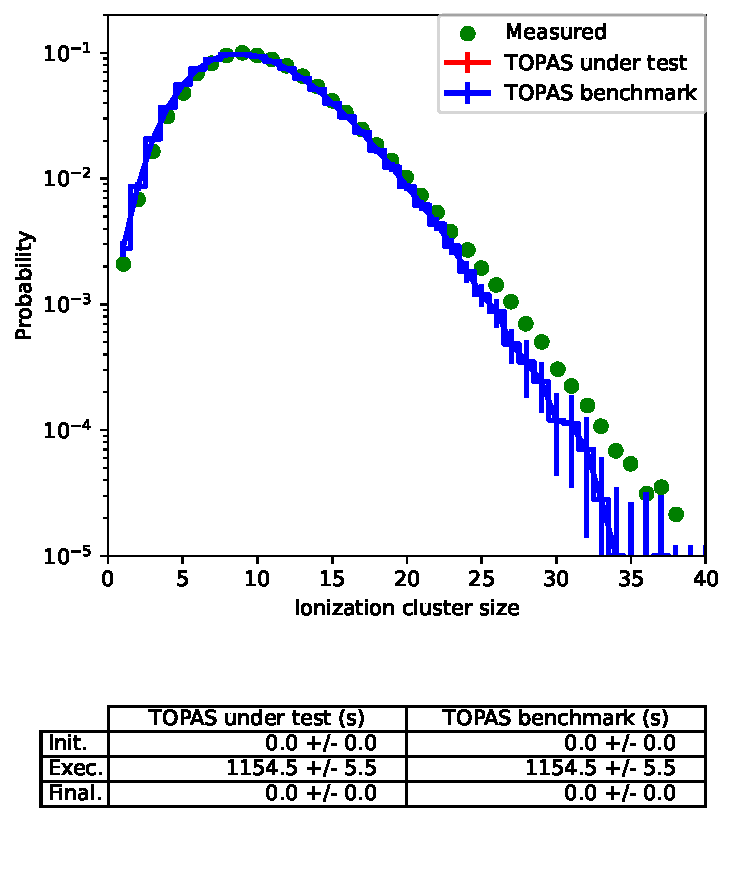
\includegraphics[width=\textwidth]{./nano1/IDDistribution_opt2}
    \end{column}
   \end{columns}
\begin{itemize}
\item \tiny{Conte V, Selva A, Colautti P, et al., Nanodosimetry: Towards a new concept of radiation quality. \textit{Radiat Prot Dosimetry}. 2018;180(1-4):150-156. doi:10.1093/rpd/ncx175}
\end{itemize}
\end{frame}

\section{Nanodosimetry I: g4em-dna\_opt4 and g4em-dna\_opt6}

\begin{frame}{\secname}
  \begin{columns}
    \begin{column}{0.4\linewidth}
     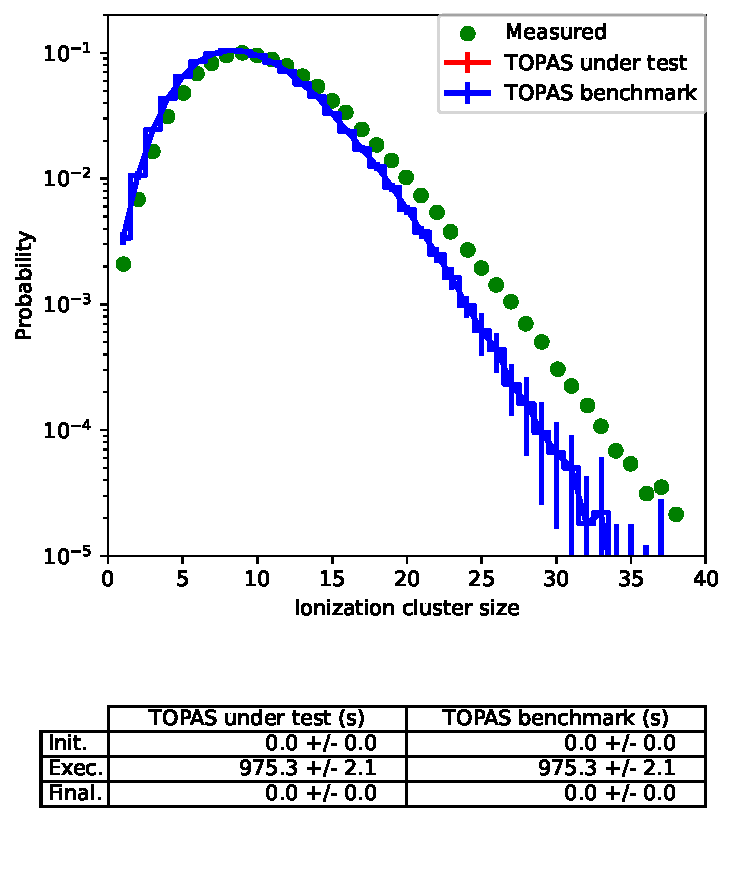
\includegraphics[width=\textwidth]{./nano1/IDDistribution_opt4}
    \end{column}
    \begin{column}{0.4\linewidth} 
     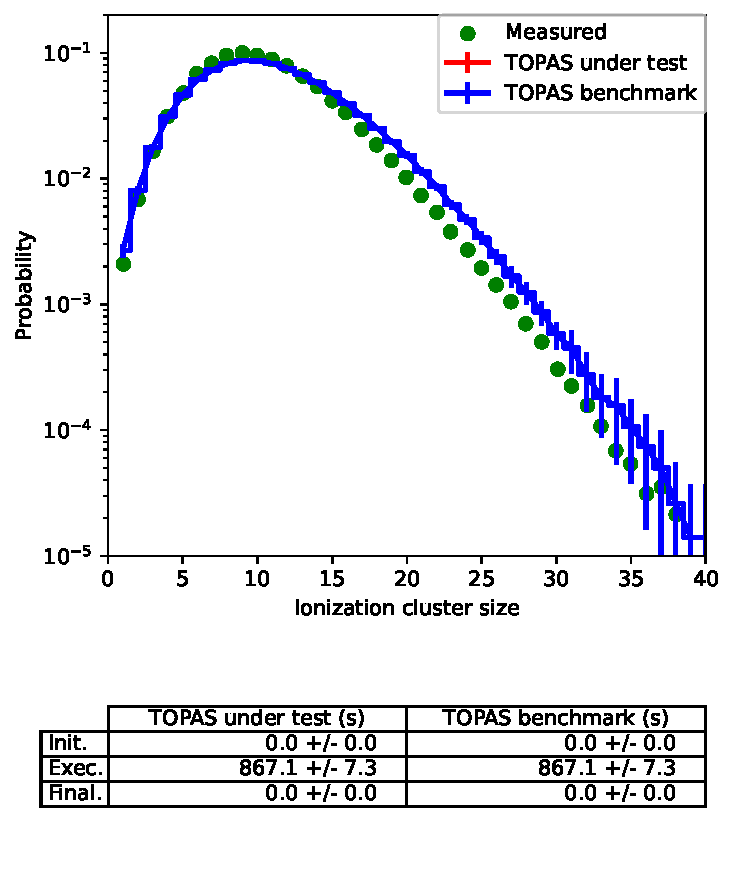
\includegraphics[width=\textwidth]{./nano1/IDDistribution_opt6}
    \end{column}
   \end{columns}
\begin{itemize}
\item \tiny{Conte V, Selva A, Colautti P, et al., Nanodosimetry: Towards a new concept of radiation quality. \textit{Radiat Prot Dosimetry}. 2018;180(1-4):150-156. doi:10.1093/rpd/ncx175}
\end{itemize}
\end{frame}

\section{Nanodosimetry II: TsEmDNAPhysics and g4em-dna\_opt2}

\begin{frame}{\secname}
  \begin{columns}
    \begin{column}{0.4\linewidth}
     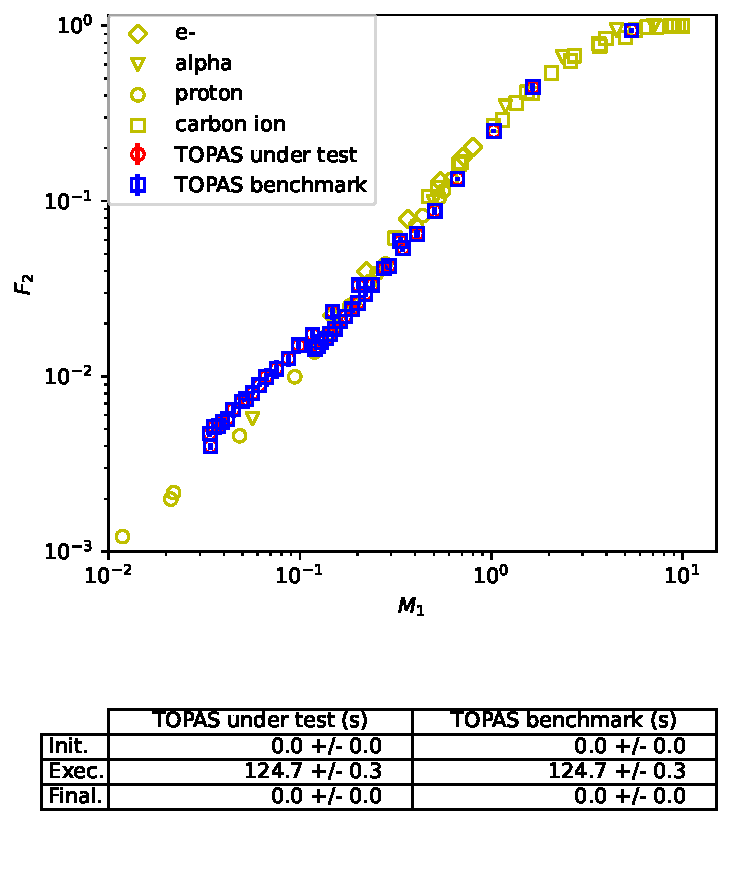
\includegraphics[width=\textwidth]{./nano2/nanoII_TsEMDNAPhysics}
    \end{column}
    \begin{column}{0.4\linewidth} 
     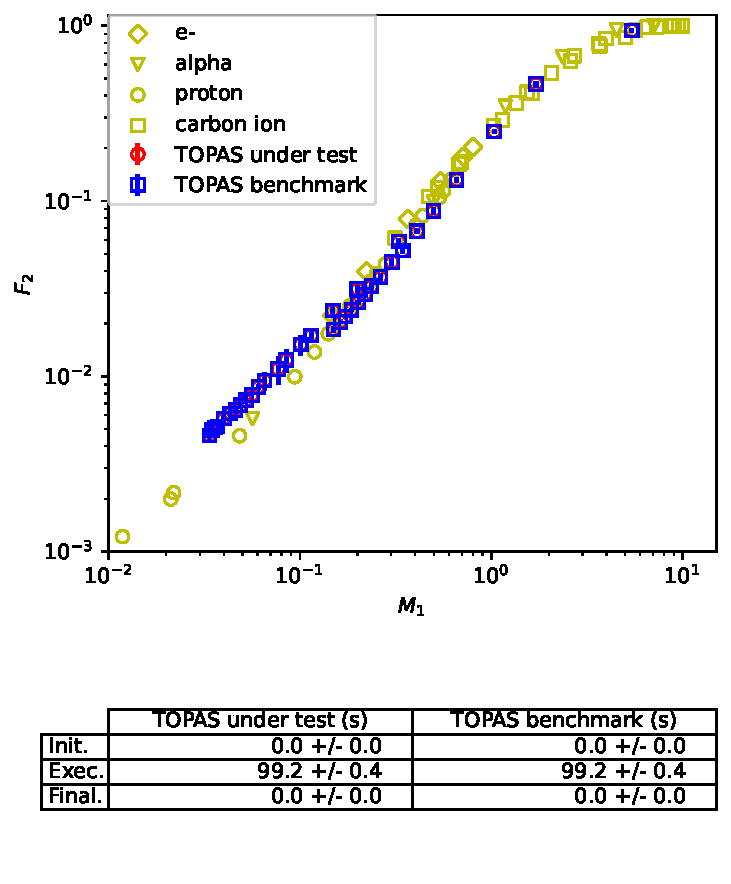
\includegraphics[width=\textwidth]{./nano2/nanoII_opt2}
    \end{column}
   \end{columns}
\begin{itemize}
\item \tiny{Conte V, Selva A, Colautti P, et al., Nanodosimetry: Towards a new concept of radiation quality. \textit{Radiat Prot Dosimetry}. 2018;180(1-4):150-156. doi:10.1093/rpd/ncx175}
\end{itemize}
\end{frame}

\section{Nanodosimetry II: g4em-dna\_opt4 and g4em-dna\_opt6}

\begin{frame}{\secname}
  \begin{columns}
    \begin{column}{0.4\linewidth}
     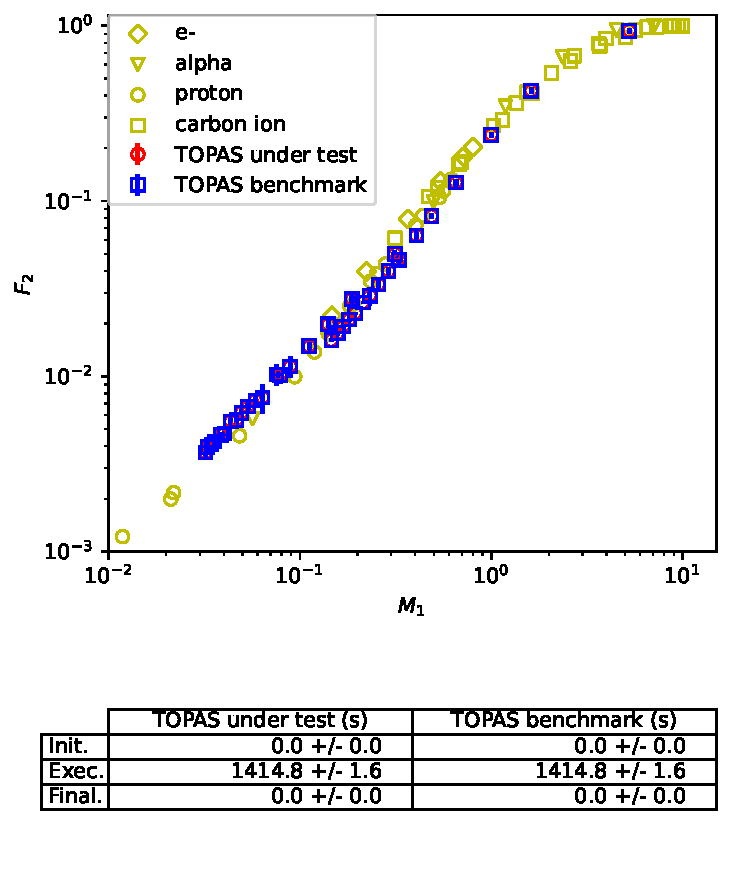
\includegraphics[width=\textwidth]{./nano2/nanoII_opt4}
    \end{column}
    \begin{column}{0.4\linewidth} 
     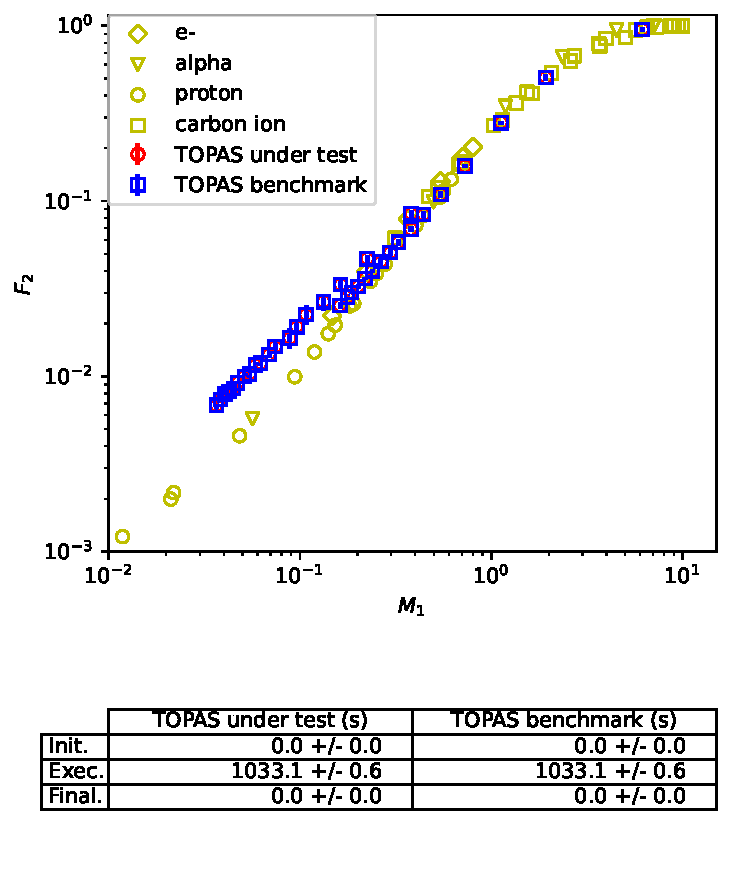
\includegraphics[width=\textwidth]{./nano2/nanoII_opt6}
    \end{column}
   \end{columns}
\begin{itemize}
\item \tiny{Conte V, Selva A, Colautti P, et al., Nanodosimetry: Towards a new concept of radiation quality. \textit{Radiat Prot Dosimetry}. 2018;180(1-4):150-156. doi:10.1093/rpd/ncx175}
\end{itemize}
\end{frame}

\section{Nanodosimetry III: TsEmDNAPhysics}

\begin{frame}{\secname}
 \centering
   \includegraphics[width=0.75\textwidth]{./nano3/nanoIII_TsEMDNAPhysics}
\begin{itemize}
 \item \tiny{Ramos-M\'endez J, Burigo LN, Schulte R, Chuang C, Faddegon B. Fast calculation of nanodosimetric quantities in treatment planning of proton and ion therapy. \textit{Phys Med Biol.} 2018;63(23):235015. doi:10.1088/1361-6560/aaeeee}
\end{itemize}
\end{frame}

\section{Nanodosimetry III: g4em-dna\_opt2}

\begin{frame}{\secname}
 \centering
   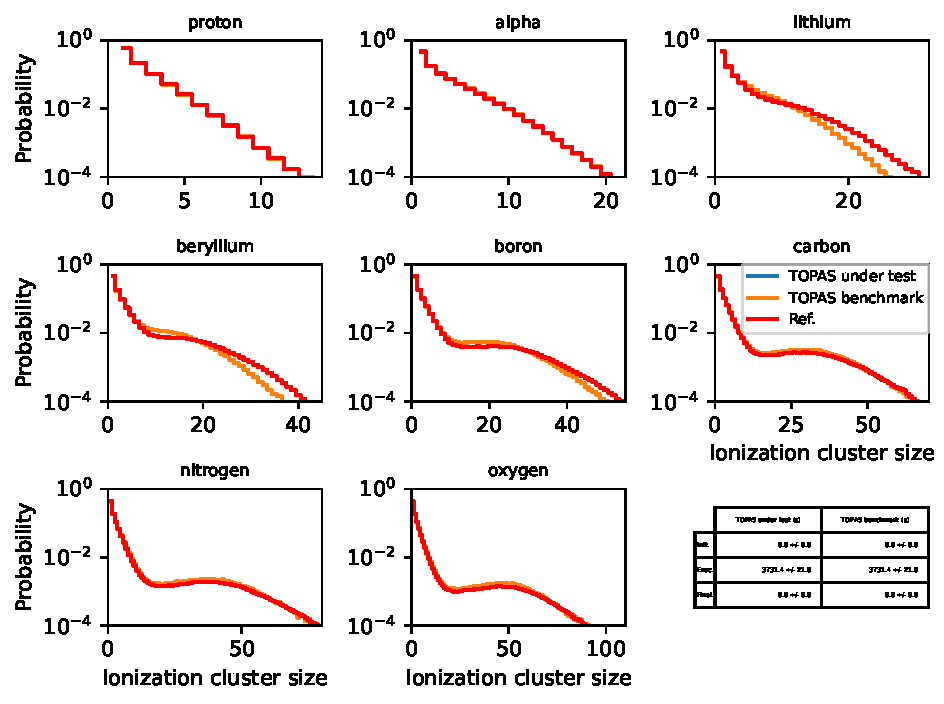
\includegraphics[width=0.75\textwidth]{./nano3/nanoIII_opt2}
\begin{itemize}
 \item \tiny{Ramos-M\'endez J, Burigo LN, Schulte R, Chuang C, Faddegon B. Fast calculation of nanodosimetric quantities in treatment planning of proton and ion therapy. \textit{Phys Med Biol.} 2018;63(23):235015. doi:10.1088/1361-6560/aaeeee}
\end{itemize}
\end{frame}

\section{Nanodosimetry III: g4em-dna\_opt4}

\begin{frame}{\secname}
 \centering
   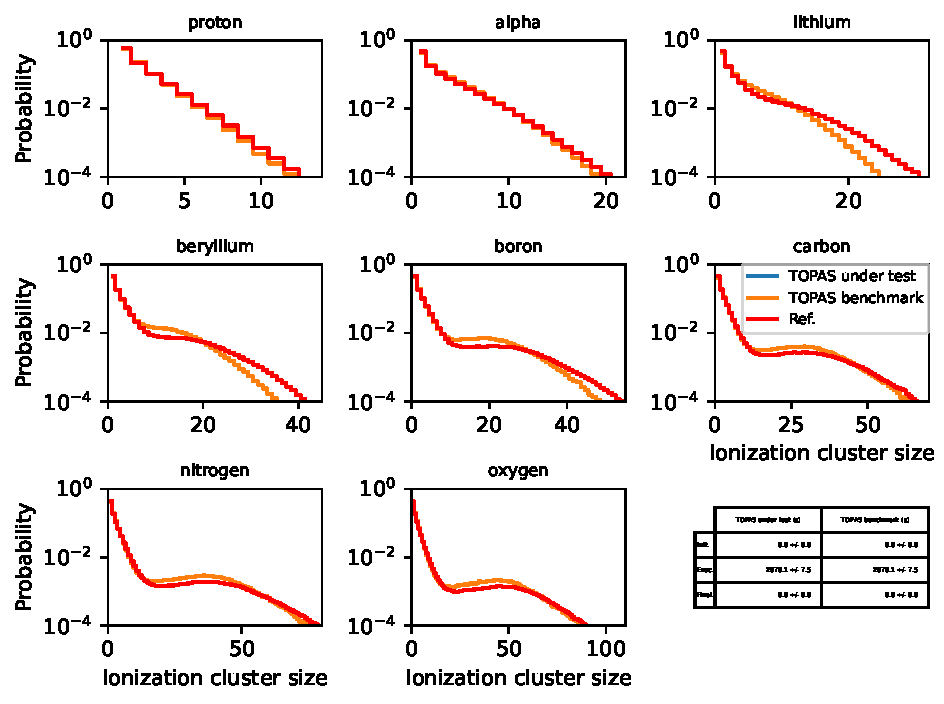
\includegraphics[width=0.75\textwidth]{./nano3/nanoIII_opt4}
\begin{itemize}
 \item \tiny{Ramos-M\'endez J, Burigo LN, Schulte R, Chuang C, Faddegon B. Fast calculation of nanodosimetric quantities in treatment planning of proton and ion therapy. \textit{Phys Med Biol.} 2018;63(23):235015. doi:10.1088/1361-6560/aaeeee}
\end{itemize}
\end{frame}

\section{Nanodosimetry III: g4em-dna\_opt6}

\begin{frame}{\secname}
 \centering
   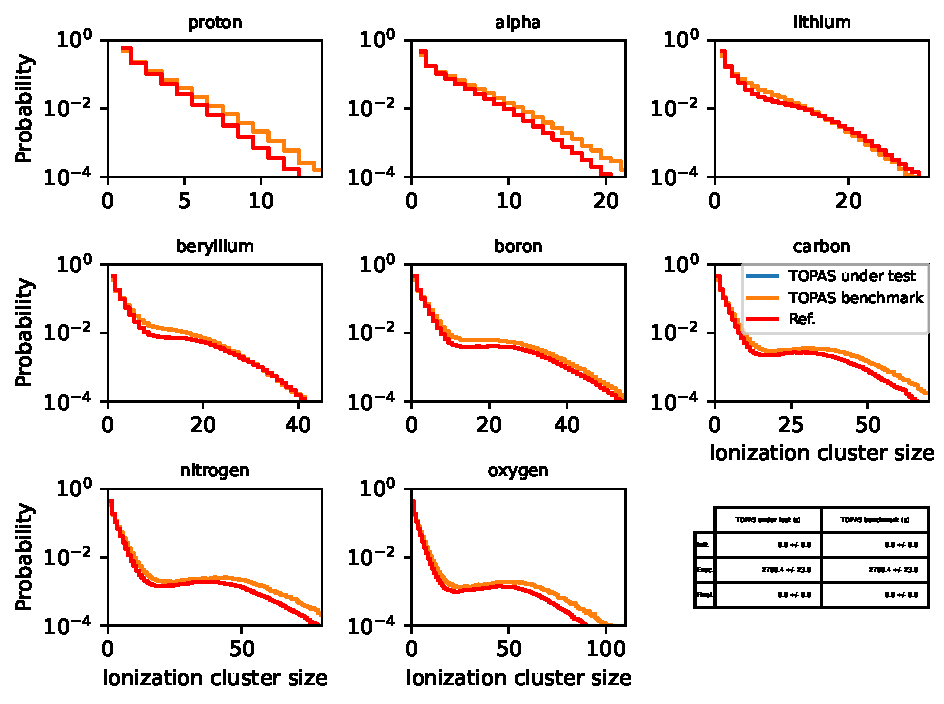
\includegraphics[width=0.75\textwidth]{./nano3/nanoIII_opt6}
\begin{itemize}
 \item \tiny{Ramos-M\'endez J, Burigo LN, Schulte R, Chuang C, Faddegon B. Fast calculation of nanodosimetric quantities in treatment planning of proton and ion therapy. \textit{Phys Med Biol.} 2018;63(23):235015. doi:10.1088/1361-6560/aaeeee}
\end{itemize}
\end{frame}

\end{document}
